\documentclass[12pt,twoside]{article}
\usepackage[utf8]{inputenc}

\usepackage{amsthm}
\theoremstyle{plain}

\usepackage{amsmath}
\usepackage[utf8]{inputenc}
\usepackage[english]{babel}
\usepackage[backend=bibtex,style=alphabetic]{biblatex}
\usepackage{hyperref}
\usepackage[margin={1.2in,1.2in},footskip=0.5in]{geometry}
\usepackage{graphicx}
\usepackage{float}
\usepackage{amssymb}
\usepackage{bbm}
\usepackage{xcolor}
\usepackage{graphicx}
\usepackage{enumerate}
\usepackage{titlesec}

\setlength{\parindent}{0pt}
\setlength{\parskip}{10pt}
\renewcommand{\baselinestretch}{1.2}

\newcommand{\sectionbreak}{\clearpage}

\theoremstyle{plain}
\newtheorem{proposition}{Proposition}[section]
\newtheorem{lemma}[proposition]{Lemma}
\newtheorem{theorem}[proposition]{Theorem}
\newtheorem{corollary}[proposition]{Corollary}

\theoremstyle{definition}
\newtheorem{definition}[proposition]{Definition}

\theoremstyle{remark}
\newtheorem{remark}[proposition]{Remark}

\numberwithin{equation}{section}

\addbibresource{master.bib}

\begin{document}
\pagenumbering{roman}

\begin{titlepage}

\begin{center}

    {\LARGE{\bf Saddlepoint approximation of the\\
    \vspace{7pt}
    Rough Heston model}} \vspace{0.5cm}


    {\normalsize Master's Thesis submitted to}\\\vspace{0.5cm}
    
    {\large{\bf Prof. Dr. Peter K. Friz}} \\
    \vspace{5pt}
    {\large{\bf Prof. Dr. Peter Bank}} \\\vspace{0.5cm}
    {\normalsize
    Faculty II – Mathematics and Natural Sciences  \\
    Institute of Mathematics} \vspace{0.5cm}
    
    
    {\normalsize{\bf Technische Universität Berlin}} \\\vspace{1.5cm}
    
    \begin{figure}[H] 
\begin{center}

\includegraphics[scale=0.3]{TU.png}
\label{fig:tu_logo}
\end{center}
\end{figure}
    
    


    {\normalsize by \\\vspace{0.5cm}
    {\Large{\bf Konstantins Starovoitovs}} \\ \vspace{5pt}
    399241} \vspace{1cm}


    {\normalsize in partial fulfillment of the requirements
    for the degree of \\
    {\bf Master of Science in Mathematics} \\\vspace{1cm}
    June 28, 2020 \\\vspace{5pt}Berlin}

\end{center}

\end{titlepage}

\newpage\null\thispagestyle{empty}\newpage

\renewcommand{\baselinestretch}{1.0}\normalsize
\tableofcontents
\renewcommand{\baselinestretch}{1.2}\normalsize

\newpage

\renewcommand{\abstractname}{Zusammenfassung}

\begin{abstract}
    In dieser Masterarbeit führen wir die asymptotische Analyse von dem Rough Heston Modell durch. Wir bedienen uns der Tatsache, dass die charakteristische Funktion im Rough Heston Modell aus der Lösung einer Volterra-Integralgleichung gewonnen werden kann. Wir untersuchen die asymptotische Entwicklung der Lösung der genannten Integralgleichung, um das asymptotische Verhalten der Randdichte für extreme Werte des Preises herzuleiten. Darauffolgend nutzen wir die Asymptotik der Randdichte, um auf das Verhalten der Preise europäischer Call-Optionen und der implizierten Black–Scholes Volatität für extreme Werte von Strike zu schließen. Das resultierende Verhalten zeigt eine Verbesserung der Näherung der implizierten Volatilität für extreme Werte von Strike. Das resultierende Verhalten zeigt eine Verbesserung der Näherung der implizierten Volatilität für extreme Werte vom Strike.
\end{abstract}

\newpage

\setcounter{page}{1}
\pagenumbering{arabic}

\section{Introduction}

In the past decade the financial industry underwent a major paradigm shift. In response to the subprime mortgage crisis of the late 2000s and resulting regulatory constraints, focus of the researchers and practitioners has moved from the asset pricing perspective to the issues concerned with risk management \cite{BW14}. This developement has increased the demand for more accurate models. In this regard we consider the novel Rough Heston model introduced in \cite{ER16}. The Rough Heston model is the ``rough'' modification of the classical Heston model, meaning that the variance process is driven by the fractional Brownian motion with Hurst index $H<\frac 12$. The model features realistic asset price dynamics and allows for refined modelling of the volatility smile.

In this thesis we set out the objective to derive a refined asymptotic expansion of the marginal density $D_T(x)$ in the Rough Heston model. We study the asymptotic behavior of $D_T(x)$ at extreme values of the spot ($\log x \rightarrow \pm \infty$). Subsequently, we aim to translate the results onto the wing behavior of other model outputs of interest, such as call prices and implied volatility surface.

We largely follow the approach from \cite{FGGS10}, where the density asymptotics has been studied in the case of the classical Heston model. We briefly outline the method employed in \cite{FGGS10}. In the classical Heston model logarithm of the moment-generating function of the log-spot $m(s, T) = \log \mathbb E[e^{s \log S_T}]$ for a fixed moment $s \in \mathbb R$ can be obtained from the solution of an ordinary differential equation of Riccati type. Moreover, for a particular subset of the parameter space of the classical Heston model the function $m(s,T)$ explodes in finite time. Thus one can define critical moments

\begin{equation}
\label{eq: intro finite moments}
\begin{aligned}
s_+(T) =\sup \left\{u \in \mathbb{R}: \mathbb{E}\left[e^{u \log S_{T}}\right]<\infty\right\} & < +\infty \\
s_-(T) =\inf \left\{u \in \mathbb{R}: \mathbb{E}\left[e^{u \log S_{T}}\right]<\infty\right\} & > -\infty.
\end{aligned}
\end{equation}

Based on the above, the asymptotic expansion of $m(s, T)$ near the blow-up is obtained in \cite{FGGS10} by applying ODE techniques to the Riccati equation. Thereafter, one recovers asymptotic expansion of the density with the saddlepoint method applied to the Mellin transform of $m(s, T)$.

At the core of the analysis is finitude of the moment explosion times \eqref{eq: intro finite moments} in the classical Heston model. Moreover, authors in \cite{FGGS10} point out that the analysis is solely based on affine principles associated with the Heston model and thus lends itself to other models which exhibit similar structure. Observing that the Rough Heston model exhibits affine structure akin to the classical Heston model, it seems natural to generalize the ansatz to the Rough Heston model, which incorporates the classical Heston model as a special case.

However, analysis of the Rough Heston model poses technical challenges. The moment-generating function in the Rough Heston model is characterized by a solution of a \emph{fractional} Riccati equation, as opposed to the \emph{ordinary} differential equation in the classical case. One of the limitations of the fractional calculus is absence of an elementary chain rule. It renders ODE techniques from \cite{FGGS10} not applicable and raises demand for a different asymptotic expansion approach. Thus we incorporate an ansatz inspired by \cite{RO96} which entails passage to the Volterra integral equation. One then recovers asymptotic expansion of the solution near the blow-up from poles in the Mellin domain. Noting from \cite{GGP18} that finite moments in the Rough Heston model behave in a way similar to the classical Heston case, we then implement the saddlepoint method for the Rough Heston density along the lines of \cite{FGGS10}.

The rest of the thesis is structured as follows. In Section \ref{sec: preliminaries} we briefly summarize some mathematical tools which will prove useful in our analysis. In Section \ref{sec: rough heston model} we introduce the Rough Heston model and outline its defining features. In Section \ref{sec: expansion of the rough heston density} we derive asymptotics of the Rough Heston density. In Section \ref{sec: extrapolation analytics} we apply the asymptotic expansion of the density to the call price and implied volatility asymptotics. In Section \ref{sec: numerical illustration} we showcase the results with a numerical illustration. In Section \ref{sec: conclusion} we state concluding remarks.

\section{Preliminaries}
\label{sec: preliminaries}

In this section we overview some mathematical tools which we will utilize in what follows. We outline basics of the fractional calculus, the Parseval formula for the Mellin transforms, the Cauchy integral formula and relations which hold for the Gaussian hypergeometric function. Other structures and methods not revisited in this section will be defined at the place of their direct application.

\subsection{Fractional calculus}

A key step in the passage from the classical Heston model to the Rough Heston model is substitution of the classical derivative operator in the Riccati equation with the fractional one. In this regard we review some fundamentals of fractional calculus.

\begin{definition}

Let $f: \mathbb R_+\rightarrow \mathbb R$ be a function defined on the positive real numbers. The \emph{Riemann–Liouville fractional integral operator} $I^\alpha f(t)$ and \emph{fractional derivative operator} $D^\alpha f(t)$ of order $\alpha\in(0, 1]$ are given by

$$
\begin{aligned}
I^{\alpha} f(t)&=\frac{1}{\Gamma(\alpha)} \int_{0}^{t}(t-s)^{\alpha-1} f(s) ds \\[10pt]
D^{\alpha} f(t)&=\frac{1}{\Gamma(1-\alpha)}\left( \frac{d}{d t} \right) \int_{0}^{t}(t-s)^{-\alpha} f(s) d s.
\end{aligned}
$$

\end{definition}

\vspace{5pt}

As manifested in the following identities, fractional integration and fractional differentiation act in a predictable way on the power function.

\begin{proposition}

For $\alpha \in(0, 1]$ it holds

\begin{equation}
\label{eq: fractional derivatives of powers}
\begin{aligned}
I^{\alpha} t^{\nu}=t^{\nu+\alpha} \frac{\Gamma(\nu+1)}{\Gamma(\nu+\alpha+1)} & \qquad\text { for } \nu>-1 \\[10pt]
D^{\alpha} t^{\nu}=t^{\nu-\alpha} \frac{\Gamma(\nu+1)}{\Gamma(\nu-\alpha+1)} & \qquad\text { for } \nu>-1+\alpha
\end{aligned}
\end{equation}
\end{proposition}

In classical calculus one way to look at the exponential function $f(x) = C \exp(ax)$ with $a, C \in \mathbb R$ is by saying that it is the function whose derivative is proportional to the function itself. The fractional equivalent of this statement involves special functions called Mittag–Leffler functions.

\begin{definition}

For $z \in \mathbb C$ and parameters $\alpha, \beta \in \mathbb C$ the Mittag–Leffler function $E_{\alpha, \beta}$ is defined by

$$
E_{\alpha, \beta}(z)=\sum_{n = 0} ^\infty \frac{z^{n}}{\Gamma(\alpha n+\beta)}.
$$

Note that $E_{1,1}\equiv \exp$.

\end{definition}

Finally, we present the variation of the constant formula for the fractional derivative operator. The proof of the following proposition can be found in \cite{P99}.

\begin{proposition}
\label{eq: fractional variation of constant}

Let $h$ be a continuous function, $\alpha \in(0,1]$ and $\gamma \in \mathbb R$. Then the initial value problem

$$
\begin{aligned}
D^{\alpha} C(t)&=\gamma C(t)+h(t) \\[10pt]
I^{1-\alpha} C(0)&=0
\end{aligned}
$$

has a unique continuous solution

$$
C(t)=\int_{0}^{t}(t-s)^{\alpha-1} E_{\alpha, \alpha}\left(\gamma(t-s)^{\alpha}\right) h(s) ds.
$$

Additionally, for constant $h(s)\equiv \theta$, $\gamma < 0$ and $\alpha \in [0,1]$ the solution satisfies

$$
0 \leq I^\alpha C(t) \leq K
$$

for some positive constant $K$.

\end{proposition}

\subsection{Mellin transform}
\label{sec: mellin transform}

In our analysis we will encounter the Mellin transform in two contexts.
First, we will apply the Parseval formula for the Mellin transforms to the fractional Riccati equation in order to analyze its blow-up behavior. Subsequently, we will recover the Rough Heston density from the moment-generating function of the log-spot via the Mellin inversion formula. We start with the definition of the Mellin transform.

\begin{definition}
For a complex number $z \in \mathbb C$ the \emph{Mellin transform} of a function $f: \mathbb{R}_{+} \rightarrow \mathbb{R}$ is given by
\begin{equation}
\label{eq: mellin transform}
M[f(x); z] := \int_{0}^{\infty} x^{z-1} f(x) d x.
\end{equation}

\end{definition}

It is apparent from the definition of the Mellin transform that it generally does not exist for all values of $z\in \mathbb C$. This motivates the following definition.

\begin{definition}
The open strip $\left\{z \in \mathbb C: \alpha < \Re (z) < \beta\right\}$ where

$$
\begin{aligned}
\alpha &= \inf\{u \in \mathbb R : f = O(t^{-u}) \text{ as } t \rightarrow 0\} \\[5pt]
\beta &= \sup\{u \in \mathbb R : f = O(t^{-u}) \text{ as } t \rightarrow +\infty\}
\end{aligned}
$$

is called the \emph{fundamental strip} or \emph{strip of analyticity} of $M[f(x); z]$.
\end{definition}

The definition implies that strip of analyticity of the Mellin transform $M[f(x);z]$ is characterized by the asymptotic behavior of the function $f$ at the limits $t\rightarrow 0$ and $t\rightarrow +\infty$. Another simple consequence from the definition of the Mellin transform is its scale invariance.

\begin{proposition}

For $\eta \in \mathbb R$ the Mellin transform satisfies

\begin{equation}
\label{eq: mellin scale invariance}
M[f(\eta x); z] = \eta^{-z} M[f(x); z].
\end{equation}

\end{proposition}

We next introduce the Mellin inversion formula.

\begin{proposition}

Consider the Mellin transform $M[f(x); z]$ of a piecewise continuous function $f: \mathbb{R}_{+} \rightarrow \mathbb{R}$ with the fundamental strip $\alpha<\Re (z)<\beta$. Assume it additionally satisfies

\begin{itemize}
    \item $M[f(x); z]$ is absolutely convergent in the fundamental strip;
    \item For all $\alpha<\Re (z)<\beta$ the Mellin transform $M[f(x); z]$ converges uniformly to zero as $\Im(z)\rightarrow \pm \infty$.
\end{itemize}

Then for any $\gamma \in\mathbb R$ with $\alpha < \gamma < \beta$ the \emph{Mellin inversion formula} holds

\begin{equation}
\label{eq: mellin inversion formula}
f(x)=\frac{1}{2 \pi i} \int_{\gamma-i \infty}^{\gamma+i \infty} M[f(\cdot); z] x^{-z} \mathrm{d} z.
\end{equation}

\end{proposition}

In conclusion, we state the Parseval formula for the Mellin transforms reminiscent of the Plancherel theorem for the Fourier transforms.

\begin{proposition}

Assume that $f, g:\mathbb R_+\rightarrow \mathbb R$ are functions such that their Mellin transforms exist and 

$$\int_{0}^{\infty} f(t) g(t) d t < \infty.$$

For $\gamma\in \mathbb R$ lying in the fundamental strip of both Mellin transform $M[g(\cdot);z]$ and $M[f(\cdot); 1-z]$ the \emph{Parseval formula} for Mellin transforms reads

\begin{equation}
\label{eq: parseval formula}
\int_{0}^{\infty} f(t) g(t) d t=\frac{1}{2 \pi i} \int_{\gamma-i \infty}^{\gamma+i \infty} M[g (\cdot); z] M[f (\cdot); 1-z] d z.
\end{equation}

\end{proposition}

The Mellin inversion formula \eqref{eq: mellin inversion formula} requires contour integration in the complex plane. Shifting the integration contour in the complex plane might entail computation of the contour integral around the poles. This can be done with the Cauchy integral formula.

\begin{proposition}
Let $f$ be a holomorphic function and $a \in \mathbb C$. Consider a contour $\gamma$ which encloses $a$. Then the \emph{Cauchy integral formula} holds

\begin{equation}
\label{eq: cauchy integral formula}
f^{(n)}(a)=\frac{n !}{2 \pi i} \oint_{\gamma} \frac{f(z)}{(z-a)^{n+1}} d z.
\end{equation}
\end{proposition}

\subsection{Gaussian hypergeometric function}
\label{sec: hypergeometric function}

We cite some results on the Gaussian hypergeometric function $_2 F_1$ from \cite{BCLO10}, which will arise in the analysis of the fractional integral. We start with the integral definition of the function $_2F_1$. 

\begin{definition}
Let $a,b,c,z\in \mathbb C$ such that in addition $\Re(c)>\Re(b)>0$ and denote by $\mathrm B$ the Euler beta function. The \emph{Gaussian hypergeometric function ${_2 F_1}$} is given by

\begin{equation}
\label{eq: hypergeometric integral definition}
\frac{1}{\mathrm{B}(b, c-b)} \int_{0}^{1} x^{b-1}(1-x)^{c-b-1}(1-z x)^{-a} d x = {_{2} F_{1}}(a, b ; c ; z).
\end{equation}
\end{definition}

Alternatively the function $_2F_1$ can be given in terms of the power series.

\begin{proposition}

The power series for the function $_2F_1$ reads

\begin{equation}
\label{eq: hypergeometric series definition}
\begin{aligned}
_{2} F_{1}(a, b ; c ; z)&=\sum_{n=0}^{\infty} \frac{(a)_{n}(b)_{n}}{(c)_{n}} \frac{z^{n}}{n !} \\[10pt]
(q)_{n}&=\left\{\begin{array}{ll}1 & n=0 \\ q(q+1) \cdots(q+n-1) & n>0\end{array}\right.
\end{aligned}
\end{equation}

\end{proposition}

We will also make use of th2e following relation for the function $_2F_1$.

\begin{proposition}

The hypergeometric function $_2F_1$ satisfies the relation

\begin{equation}
\label{eq: hypergeometric relation}
\begin{aligned}
_2F_1(a,b,c;z) &= \frac{\Gamma(a+b-c) \Gamma(c)}{\Gamma(a) \Gamma(b)}(1-z)^{c-a-b}{_{2} F_{1}}(c-a, c-b ; c-a-b+1 ; 1-z) \\[10pt]
&\qquad +\frac{\Gamma(c-a-b) \Gamma(c)}{\Gamma(c-a) \Gamma(c-b)} {_2 F_{1}}(a, b ; a+b-c+1 ; 1-z).
\end{aligned}
\end{equation}
\end{proposition}

% \subsection{saddlepoint method}

% We start by considering Laplace's method and then proceed to its complex-analytic analogue which is the saddlepoint method. The Laplace's method is a technique to approximate integrals of the form $\int_{a}^{b} e^{M f(x)} d x$ where $M$ is very large. The idea is to reduce calculation of the integral to the simpler one that can be explicitly evaluated (asymptotically). For a smooth function which takes global maximum at a point at the point $x_0$, we can write

% $$
% \int_{a}^{b} e^{M f(x)} d x \approx e^{M f\left(x_{0}\right)} \int_{a}^{b} e^{-\frac{1}{2} M\left|f^{\prime \prime}\left(x_{0}\right)\right|\left(x-x_{0}\right)^{2}} d x =\sqrt{\frac{2 \pi}{M\left|f^{\prime \prime}\left(x_{0}\right)\right|}} e^{M f\left(x_{0}\right)}
% $$

% due to Taylor expansion, $f'(x_0) = 0$ and the fact that the last integral is Gaussian.

% The saddlepoint method generalizes the method to the contour integrals in the complex plane.

\section{Rough Heston model}
\label{sec: rough heston model}

The celebrated Black–Scholes model is the simplest asset pricing model that laid the foundation for option pricing theory \cite{BS73}. In the Black–Scholes model the spot process $S_t$ under the risk-neutral measure follows log-normal dynamics

\begin{equation}
\label{eq: black scholes}
\frac{dS_t}{S_t} = r dt + \sigma dW_t,
\end{equation}

where $r$ is the risk-free rate, $\sigma$ is the annualized constant volatility of the returns and $W_t$ is the standard Brownian motion. Despite its omnipresence in the financial world, the Black–Scholes model is not consistent with the market. Contrary to the assumptions of the Black–Scholes model, volatility surfaces implied from the market prices of liquid vanilla instruments are not flat and exhibit volatility smile \cite{DK94}.

In order to capture the volatility smile one can expand the Black–Scholes model to general Markovian setting and introduce dependence of the volatility $\sigma$ in \eqref{eq: black scholes} on time $t$ and the asset price process $S_t$. This leads to the class of \textit{local volatility models} introduced in \cite{D94}, where the volatility process reads $\sigma(t, S_t)$. While such models manage to accommodate the entire volatility smile and are actively used in the valuations of exotic derivatives, dynamic evolution of the market smile in local volatility models is inconsistent with the market. When the price of the spot increases, local volatility models predict that the market smile shifts to lower prices and vice versa \cite{HKLW02}. This contradicts the typical market behavior: the smiles move in the same direction as the underlying. This discord between the market and the model leads to incorrect hedges derived from the local volatility models.

In addition, empirical studies of asset price dynamics in the past decades accumulated statistical evidence for a number of universal properties associated with asset returns that used to be part of the market folklore \cite{C01}. These properties are commonly referred to as ``stylized facts'' and are expected to be reproduced by any reasonable asset pricing model. Some of the most prominent of them are
\clearpage
\begin{enumerate}[(i)]
    \item \emph{Fat tails.} The tails of the marginal returns distribution are heavier when compared to normal distribution \cite{M67}.
    \item \emph{Volatility clustering.} Tendency of large price fluctuations to be followed by large price fluctuations of either sign \cite{M67}.
    \item \emph{Leverage effect.} Negative relation between the movements of volatility and spot \cite{C82}.
    \item \emph{Time-varying volatility} \cite{C01}.
\end{enumerate}

A natural way to accommodate the above features while retaining Markoviantity is equipment of the model with another stochastic factor. Models in which the volatility process $\sigma_t$ admits its own source of randomness form a class of \textit{stochastic volatility models}. One of the most popular stochastic volatility models is the renowned Heston stochastic volatility model \cite{H93}. The Heston model is a stochastic volatility model where the variance process follows mean-reverting CIR process. Specifically, dynamics in the Heston model is given by

\begin{equation}
\label{eq: heston SDEs}
\begin{aligned}
d S_{t}&=S_{t} \sqrt{V_{t}} d W_{t} \\[5pt]
d V_{t}&=\lambda\left(\bar v-V_{t}\right) d t+\xi \sqrt{V_{t}} d B_{t} \\[5pt]
\langle dW_t, dB_t\rangle &= \rho dt.
\end{aligned}
\end{equation}

\vspace{10pt}

Table \ref{table: heston parameters} summarizes parametrization of the Heston model \eqref{eq: heston SDEs}.

\vspace{10pt}

\begin{table}[H]
\centering
\begin{tabular}{r l c}
    \hline
    Parameter & Interpretation & Constraint \\
    \hline\hline
    $v_0$ & initial variance & $v_0 > 0$ \\
    $\bar v$ & long-term mean variance & $\bar v > 0$ \\
    $\lambda$ & mean-reversion speed & $\lambda > 0$ \\
    $\xi$ & volatility of volatility & $\xi > 0$ \\
    $\rho$ & spot-variance correlation & $-1 \leq \rho \leq 1$ \\
    \hline
\end{tabular}
\caption{Parameters of the Heston model.}
\label{table: heston parameters}
\end{table}

\vspace{20pt}

\newpage

A defining feature of the Heston model is its \emph{affine structure}: in the original paper \cite{H93} the moment-generating function is obtained from \eqref{eq: heston SDEs} by considering affine ansatz for the Itô differential of $\mathbb{E}\left[e^{s \log S_{T}} | \mathcal{F}_{t}\right]$ for the filtration $\mathcal{F}_{t}=\sigma\left(W_{s}, B_{s} ; s \leq t\right)$. Ultimately, one obtains the moment-generating function $\mathbb{E}\left[e^{s \log S_{T}}\right]$ from solution $\psi$ of the ordinary differential equation with boundary condition

\begin{equation}
\label{eq: heston logarithm of moment-generating function}
m(s, t) = \log \mathbb{E}\left[e^{s \log S_{t}}\right]=\bar{v} \lambda I^{1} \psi(s, t)+v_{0} \psi(s, t) 
\end{equation}

\begin{equation}
\label{eq: heston riccati}
\begin{aligned}
\dot \psi(s,t) &= R(s, \psi(s, t)) \\
\psi(\cdot, 0) &= 0 \\[10pt]
R(s, w) &= \frac{1}{2}\left(s^{2}-s\right)+(\rho \xi s - \lambda) w+\frac{1}{2} \xi ^{2} w^{2}.
\end{aligned}
\end{equation}

\vspace{10pt}

There are several reasons why the Heston model has become a mainstay of the financial industry:

\begin{itemize}
    \item
    \textit{Conformance with the stylized facts from low-frequency price data.} The Heston model exhibits leverage effect, time-varying volatility and fat tails \cite{DY02}.
    \item
    \textit{Reasonable shapes for the generated implied volatility surfaces.} Volatility of volatility $\xi$ controls convexity of the smile, spot-variance correlation $\rho$ controls the skewness, baseline variance level $v_0$ fixes at-the-money volatility level \cite{FJL12}.
    \item \textit{Consistent dynamics of the implied volatility.} Volatility smile moves in the same direction as the asset price \cite{G11}.
    \item 
    \textit{Tractability of the model.} The ordinary differential equation of Riccati type \eqref{eq: heston riccati} is explicitly solvable. This leads to explicit formula for the characteristic function \cite{H93}. The closed-form characteristic function in turn induces explicit pricing formulae with transform methods and instantaneous model calibration with fast Fourier transform algorithm à la Carr–Madan \cite{L05, CM99}.
\end{itemize}

However, the Heston model, along with other classical stochastic volatility models driven by the standard Brownian motion, fails to capture risk of large price movements for short maturities \cite{J19}. Thus the generated European option prices are not consistent with observed market prices. This can be remediated by considering the novel class of ``rough'' volatility models, where the volatility is driven by the \emph{fractional} Brownian motion.

\subsection{Rough Heston model}
\label{sec: introduction rough heston model}

The key ingridient in rough volatility models is fractional Brownian motion which drives the volatility process. We briefly introduce the fractional Brownian motion and address without proof regularity of its paths. In the following we work on a filtered probability space $(\Omega, (\mathcal F_t)_{t\geq 0}, \mathbb P, \mathbb F)$ large enough to support the model in consideration.

\begin{definition}

\emph{Fractional Brownian motion} $W^H_t$ with Hurst parameter $H\in (0, 1)$ is a stochastic process with the following features:

\begin{itemize}
    \item \emph{Self-similarity.} For $a\in \mathbb R_+$ holds $\left(W_{a t}^{H}\right) \overset{law}{=} a^{H}\left(W_{t}^{H}\right)$.
    \item \emph{Stationary increments.} $\left(W_{t+h}^{H}-W_{t}^{H}\right) \overset{law}{=} \left(W_{h}^{H}\right)$.
    \item Marginal distribution of $W^H_1$ is a Gaussian random variable with $E \left[W^H_1\right] = 0$ and $E\left[(W^H_1)^2\right]=1$.
\end{itemize}

Let $W_t$ be the standard Brownian motion and $\Gamma$ the gamma function. The \emph{Mandelbrot–van Ness representation} of the fractional Brownian motion is given by

$$
W_{t}^{H}=\frac{1}{\Gamma(H+1 / 2)} \int_{-\infty}^{0}\left((t-s)^{H-\frac{1}{2}}-(-s)^{H-\frac{1}{2}}\right) d W_{s}+\frac{1}{\Gamma(H+1 / 2)} \int_{0}^{t}(t-s)^{H-\frac{1}{2}} d W_s.
$$

The \emph{Riemann–Liouville representation} of the fractional Brownian motion is given by

$$
W^H_t = \sqrt{2H} \int _0^t(t-s)^{H-\frac 12} dW_t.
$$

\vspace{5pt}

\end{definition}

\begin{remark}
For all $\varepsilon > 0$, paths of $W^H$ are $\mathbb P-\text{a.s.}$ $(H-\varepsilon)$–Hölder continuous.
\end{remark}

\begin{remark}
For $H=\frac 12$ we recover the standard Brownian motion. Paths of standard Brownian motion exhibit Hölder regularity of $\frac 12-\varepsilon$ for all $\varepsilon > 0$.
\end{remark}

Statistical analysis of ultra-high-frequency time series data performed in the seminal work \cite{GJR14} concluded that paths of the log-volatility of major market indices exhibit Hölder regularity lower than that of the standard Brownian motion. Specifically, the realized log-volatility can be accurately fitted by the fractional Brownian motion with Hurst index 0.1. Moreover, volatility models driven by the fractional Brownian motion also generate reasonable shapes of the implied volatility surfaces for short maturities. These considerations motivate introduction of the rough counterpart of the Heston model to allow for the fractional volatility driver. 

\begin{definition}

Let $(W_t, B_t)$ be the standard two-dimensional Brownian motion. For $\alpha \in \left(\frac 12, 1\right)$ we define the \emph{Rough Heston model} $(S_t, V_t)$ where the spot process $S_t$ and variance process $V_t$ obey the equations

\begin{equation}
\label{eq: rough heston model}
\begin{aligned}
d S_{t}&=S_{t} \sqrt{V_{t}} d W_{t} \\[5pt]
V_{t}&=V_{0}+\frac{1}{\Gamma(\alpha)} \int_{0}^{t}(t-s)^{\alpha-1} \lambda\left(\bar v-V_{s}\right) d s+\frac{1}{\Gamma(\alpha)} \int_{0}^{t}(t-s)^{\alpha-1} \lambda \xi \sqrt{V_{s}} d B_{s} \\[5pt]
\left\langle d W_{t}, d B_{t}\right\rangle&=\rho d t.
\end{aligned}
\end{equation}

The interpretation of the parameters is equivalent with the classical Heston model in Table~\ref{table: heston parameters}. Additional parameter $\alpha$ corresponds to the \emph{roughness} of the paths.

\end{definition}

\vspace{10pt}

\begin{remark}
For $\alpha = 1$, we recover the Heston model \eqref{eq: heston SDEs}. From now on we refer to the Heston model defined in \eqref{eq: heston SDEs} as the \emph{classical Heston model} in order to differentiate between the two.
\end{remark}

Virtually all stylized facts attributed to the behavior of volatility are recovered with the fractional driver \cite{ER16}. Moreover, rough volatility models provide a remarkable fit of the implied volatility surface for short maturities \cite{BFG16}.

However, working with the fractional Brownian motion entails technical challenges. First, the resulting variance process in \eqref{eq: rough heston model} is not a semimartingale, since it has unbounded quadratic variation, which renders Itô calculus not applicable \cite{ER16}. Moreover, the resulting process depends of the past realization of the Brownian motion and hence it is not Markovian.

\subsection{Characteristic function of the log-stock price}
\label{sec: characteristic function rough heston}

As mentioned above, a major feature of the classical Heston model is the explicit characteristic function. It turns out that the Rough Heston model exhibits similar affine structure. However, one cannot derive it by means of Itô calculus akin to the classical Heston model. The variance process in the Rough Heston model is not a semimartingale, which renders the Itô's lemma not applicable. Instead, the equation for the logarithm of moment-generating function in the Rough Heston model was established in \cite{ER16} by means of a sequence of high-frequency models based on Hawkes processes.

\begin{definition}

A \emph{two-dimensional Hawkes process} is a point process $\left(N_{t}^{+}, N_{t}^{-}\right)_{t \geq 0}$ with intensity given by

\begin{equation}
\label{eq: hawkes process}
\left(\begin{array}{c}\lambda_{t}^{+} \\ \lambda_{t}^{-}\end{array}\right)=\left(\begin{array}{c}\mu^{+} \\ \mu^{-}\end{array}\right)+\int_{0}^{t}\left(\begin{array}{cc}\varphi_{1}(t-s) & \varphi_{3}(t-s) \\ \varphi_{2}(t-s) & \varphi_{4}(t-s)\end{array}\right) \cdot\left(\begin{array}{c}d N_{s}^{+} \\ d N_{s}^{-}\end{array}\right),
\end{equation}

where $\mu^+, \mu^- \in \mathbb R$ correspond to baseline intensity level and $\varphi_i$ for $i \in \{1,2,3,4\}$ are measurable non-negative deterministic functions.

\end{definition}

Note that Hawkes process is not Markovian, since the intensity level at time $t$ depends on the entire trajectory $\left(N_{s}^{+}, N_{s}^{-}\right)_{0 \leq s \leq t}$. In the language of branching processes such process is called \textit{self-exciting}. The microstructural model of the asset price in \cite{ER16} is then simply given by

\begin{equation}
\label{eq: hawkes processes microstructure model}
P_{t}=N_{t}^{+}-N_{t}^{-}
\end{equation}

where $N_{t}^{+}$ corresponds to upward price movements and $N_{t}^{-}$ corresponds to downward price movements.

A crucial role in the construction plays the kernel matrix $\big(\begin{smallmatrix}
\varphi_1 & \varphi_3 \\ \varphi_2 & \varphi_4
\end{smallmatrix}\big)$  in the definition of the intensity of the Hawkes process in \eqref{eq: hawkes process}. The kernel matrix quantifies degree of endogeneity of the market and is thus sometimes dubbed \emph{memory kernel function}. High degree of the market endogeneity is manifested in the $L^1$-norm of the largest eigenvalue of the kernel matrix being close to unity. Liquid markets are highly \emph{endogenous}, meaning that most transactions have no economic rationale but are rather executed algorithmically in reaction to other large institutional orders or \emph{metaorders} \cite{FS12}. The metaorders are subjected to optimal execution algorithms and broken down in smaller orders.

Depending on the postulated endogeneity of the market, with appropriate scaling one obtains the Heston model \cite{JR15} or the Rough Heston model \cite{ER16} as the scaling limit of the high-frequency models \eqref{eq: hawkes processes microstructure model}. The characteristic function of the Rough Heston model is then obtained from the limiting behavior of the characteristic function of the Hawkes process. We cite the correspoding result for the Rough Heston model from \cite{ER16}.

\begin{proposition}

The logarithm of moment-generating function of the log-spot $m(s, t)$ in the Rough Heston model \eqref{eq: rough heston model} is characterized by the solution of the fractional Riccati equation:

\begin{equation}
\label{eq: logarithm of moment-generating function}
m(s, t) = \log \mathbb{E}\left[e^{s \log S_{t}}\right]=\bar{v} \lambda I^{1} \psi(s, t)+v_{0} I^{1-\alpha} \psi(s, t)
\end{equation}

\begin{equation}
\label{eq: fractional riccati formulation}
\begin{aligned}
D^\alpha\psi(s,t) &= R(s, \psi(s, t))\\
\psi(\cdot, 0) &= 0 \\[10pt]
R(s, w) &= \frac{1}{2}\left(s^{2}-s\right)+(\rho \xi s - \lambda) w+\frac{1}{2} \xi ^{2} w^{2}.
\end{aligned}
\end{equation}

\end{proposition}

Note that the equation \eqref{eq: fractional riccati formulation} is almost identical with the classical Heston case in \eqref{eq: heston riccati}, but now the ordinary differential operator is replaced with the fractional one.

At last, we cite a result from \cite{KST06} which establishes one-to-one correspondence between solutions of fractional Riccati equations and Volterra integral equations. Working with integral equations instead will prove beneficial due to application of integral transforms. Heuristically equivalence of \eqref{eq: fractional riccati formulation} with the corresponding integral equation can be seen by applying the fractional integration operator $I^{\alpha}(\cdot)$ to both sides of $\eqref{eq: logarithm of moment-generating function}$. 

\begin{proposition}
\label{prop: riccati iff volterra}

Let $\alpha \in (0, 1)$, $T>0$ and suppose that $\psi\in C[0, T]$ and $H\in C(\mathbb R)$. Then $\psi$ satisfies the fractional differential equation

$$
\begin{aligned} D_{t}^{\alpha} \psi(t) &=H(\psi(t)) \\ I_{t}^{1-\alpha} \psi(0) &=0 \end{aligned}
$$

if and only if it satisfies the Volterra integral equation

$$
\psi(t)=\frac{1}{\Gamma(\alpha)} \int_{0}^{t}(t-s)^{\alpha-1} H(\psi(s)) d s.
$$

\end{proposition}

Thus Proposition \ref{prop: riccati iff volterra} allows us to work with Volterra integral equation.

\begin{proposition}

The logarithm of moment-generating function of the log-spot $m(s, t)$ in the Rough Heston model \eqref{eq: rough heston model} is characterized by the solution of the Volterra integral equation:

\begin{equation}
\label{eq: original volterra equation}
\begin{aligned}
\psi(s,t) &= \frac{1}{\Gamma(\alpha)} \int _0^t (t-\tau)^{\alpha-1} R(s, \psi(s, \tau)) d\tau\\[10pt]
\psi(\cdot, 0) &= 0 \\
R(s, w) &= \frac{1}{2}\left(s^{2}-s\right)+(\rho \xi s - \lambda) w+\frac{1}{2} \xi ^{2} w^{2}.
\end{aligned}
\end{equation}

\end{proposition}

\subsection{Moment explosions}
\label{sec: moment explosions}

As discussed above, one of the ``stylized facts'' associated with asset returns is fat tails of the marginal distributions. This leads to the insight that moments of the asset price process in realistic models may be infinite.

\begin{definition}

For $s\in \mathbb R$ we define the \emph{critical time}

\begin{equation}
\label{eq: critical time}    
T^{*}(s):=\sup \left\{t \geq 0: \mathbb{E}\left[e^{s \log S_{t}}\right]<\infty\right\}.
\end{equation}

\vspace{10pt}

For $T>0$ we define the \emph{critical moments}

\begin{equation}
\label{eq: definition of critical moments}
\begin{aligned}
s_+(T)&:=\sup \left\{u \in \mathbb{R}: \mathbb{E}\left[e^{u \log S_{T}}\right]<\infty\right\} \\[5pt]
s_-(T)&:=\inf \left\{u \in \mathbb{R}: \mathbb{E}\left[e^{u \log S_{T}}\right]<\infty\right\}
\end{aligned}
\end{equation}

with conventions $\sup\,\{\varnothing\} = +\infty$ and $\inf\, \{\varnothing\} = -\infty$.

\end{definition}

We overview some facts on the critical time and critical moments from \cite{GGP18}.

\vspace{10pt}

\begin{proposition}
\label{prop: facts about critical moments}

Let $S_t$ be a positive martingale. Then the following holds:

\begin{enumerate}[(i)]
    \item 
    $T^*(s)$ increases for $u\leq 0$ and decreases for $u\geq 0$.
    \item
    $s_+(T)$ decreases and $s_-(T)$ increases.
    \item
    If the increase (decrease) in the above statements is strict, one function is the inverse of the other one.
\end{enumerate}

\end{proposition}

Finite critical moments are interesting for multiple reasons. First, they allow to identify convergence rate of some numerical procedures and identify the models that would assign infinite prices to particular financial products \cite{AP06}. In addition, they are important for the optimal choice of a good damping parameter in option pricing with transform methods to avoid highly oscillatory integrands, as will become apparent in Section \ref{sec: option pricing with transform methods}. We in turn follow the suit of \cite{FGGS10} and employ critical moments to study the asymptotic behavior of the implied variance.

A comprehensive study of the moment explosions in the Rough Heston model has been performed in \cite{GGP18}. We start by citing a statement relating finitude of the explosion times in the Rough Heston model and classical Heston model.

\vspace{10pt}

\begin{proposition}
\label{prop: moment explosions parameter space}

The moment $\mathbb E\left[S^s_t\right]$ for $s\in \mathbb R$  explodes in the Rough Heston model \eqref{eq: rough heston model} in finite time if and only if the moment explodes in finite time for the corresponding configuration of the classical Heston model with $\alpha=1$.

\end{proposition}

Note that while finitude of the critical time in the Rough Heston model is equivalent to the finitude of the critical time in the corresponding classical Heston model with $\alpha = 1$, the actual values of the critical time will be different in both models. The following statement from \cite{GGP18} characterizes the region of the parameter space in which a particular moment $s\in \mathbb R$ explodes.

\newpage

\begin{proposition}

The moment $s\in \mathbb R$ in the Rough Heston model \eqref{eq: rough heston model} explodes in finite time if and only if both of the following conditions are satisfied:

\end{proposition}

\begin{enumerate}[(i)]
    \item $\frac 12 s(s-1) > 0$;
    \item $
    \frac 12 (\rho \xi s - \lambda) \geq 0 \texttt{ or } \left\{ \frac 12 (\rho \xi s - \lambda) \leq 0 \texttt { and } \frac 14 (\rho \xi s - \lambda)^2 - \frac 14 \xi^2 s(s-1) <0 \right\}$.
\end{enumerate}

In our analysis, we are interested in the inverse function of the critical time – the critical moment. Finitude of the critical moments in the Rough Heston model has been also addressed in \cite{GGP18}.

\vspace{10pt}

\begin{proposition}
In the Rough Heston model the critical moments defined in \eqref{eq: definition of critical moments} are finite for every $T>0$.
\end{proposition}

It follows that while there may be moments $s\in \mathbb R$ such that the critical time $T^*(s)$ is infinite, unless conditions from Proposition \ref{prop: moment explosions parameter space} hold, the critical moment $s_+(T)$ is finite for every time $T>0$.

At last, we address calculation of the critical time and critical moments in the Rough Heston model. In the classical Heston model, owing to the closed-form characteristic function, the critical time can be calculated explicitly. The critical moments are then obtained by a root-finding procedure \cite{AP06}. Meanwhile, the Rough Heston model does not enjoy the same liberty. However, for specific configurations of the Rough Heston model the critical time can be calculated iteratively \cite{GGP18}. We thus compute the critical time and its differentials numerically. The critical moments are then obtained similarly by means of a root-finding procedure. 

Figure \ref{fig: critical moments} illustrates critical moments $s_+(T)$ in the classical Heston model and Rough Heston model with $\alpha=0.9$ and $\alpha=0.8$, respectively. Note that critical moments in the Rough Heston model are decreasing with decreasing value of $\alpha$. This signifies fatter tails in the rougher models with lower values of $\alpha$. Note also that the difference of the critical moments between the models is more pronounced for smaller time pegs, while critical moments for larger time pegs are almost equal. This manifests the ability of the Rough Heston model to capture more accurately the tail risk for short maturities.

\newpage\clearpage

\vspace{20pt}

\begin{figure}[H]
\centering
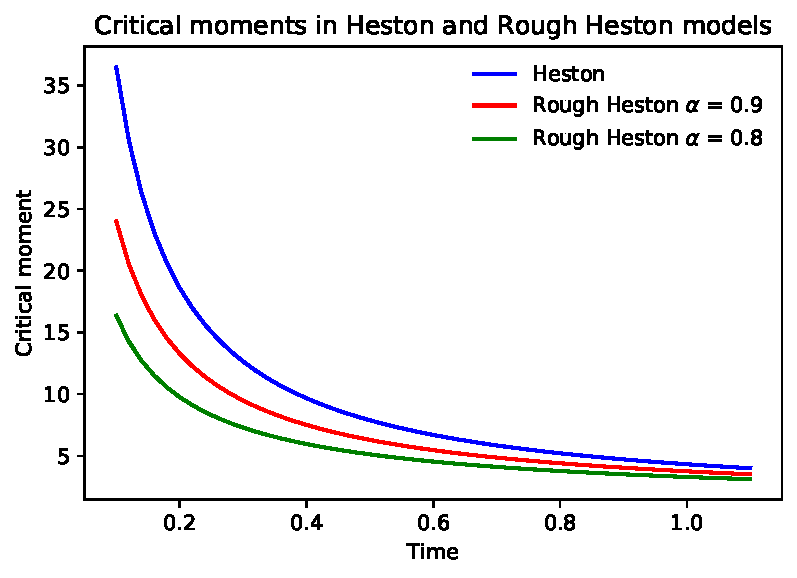
\includegraphics[width=0.7\textwidth]{figures/critical_moments.pdf} \\
\caption{Critical moments for the classical Heston model and the Rough Heston model with $\alpha=0.9$ and $\alpha=0.8$, respectively.}
\label{fig: critical moments}
\end{figure}

\section{Expansion of the Rough Heston density}
\label{sec: expansion of the rough heston density}

In this section we aim to obtain asymptotic expansion of the Rough Heston density for extreme values of the log-spot $\log x \rightarrow \pm \infty$ at a fixed timescale $T>0$.
We start by studying the blow-up behavior of the solution $\psi$ of the fractional Riccati equation in \eqref{eq: fractional riccati formulation} inspired by the procedure from in \cite{RO96}. It entails techniques from \cite{BH75} involving the Mellin transform of the integral equation. Proposition \ref{prop: blow-up behavior of the volterra integral equation} implies that for a fixed $s\in \mathbb R$ the explosive solutions $\psi(s, t)$ of the fractional Riccati equation in \eqref{eq: logarithm of moment-generating function} behave near the explosion time $T^*(s)$ as a power law $\psi(s, t) \sim (T^*(s) - t)^{-\alpha}$. Proposition \ref{prop: blow-up behavior of the volterra integral equation} relies on assumptions imposed on the solution $\psi$ of the equation \eqref{eq: fractional riccati formulation} which we summarize in the Remark \ref{remark: assumptions}.

Thereafter, we investigate the asymptotic expansion of the moment-generating function in the proximity of the critical moment. Proposition \ref{prop: explosion in terms of the critical moments} warrants singular behavior of order $m(s, t) \sim (s_+ - s)^{1-2\alpha}$ for the logarithm of the moment-generating function in terms of the critical moment $s_+$. Proposition \ref{prop: explosion in terms of the critical moments} relies on assumptions concerning the differentiability of the critical time in the Rough Heston model.

At last, we proceed along the lines of \cite{FGGS10} to obtain the asymptotic expansion of the density with the saddlepoint method. After locating the approximate saddlepoint and establishing necessary tail estimates, the refined asymptotic expansion of the density is given in Proposition \ref{prop: density main proposition}.

We will focus on the right-wing asymptotics ($\log x\rightarrow +\infty$). The analysis of the left-wing asymptotics ($\log x \rightarrow -\infty$) is completely analogous to the right-wing case. The corresponding results on the left-wing asymptotics are presented in Corollary \ref{cor: left wing expansion} at the end of the section.

\subsection{Asymptotic expansion of the fractional Riccati equation}
\label{sec: blow up behavior of fractional riccati equation}

The fractional Riccati equation \eqref{eq: fractional riccati formulation} is not solvable explicitly. As mentioned before, ODE techniques from \cite{FGGS10} used to obtain asymptotic expansion of the equation near blow-up are not applicable due to absence of an elementary chain rule for the fractional derivative. Hence we need to employ an alternative approach to expand the solution of \eqref{eq: fractional riccati formulation}.

Note that asymptotic expansion of the equation \eqref{eq: fractional riccati formulation} near $t=0$ has been obtained in \cite{GGP18} by means of a fractional power series ansatz

\begin{equation}
\label{eq: fractional power series ansatz}
\psi(s, t) \sim \sum_{n=1}^{\infty} a_{n}(s) t^{\alpha n}.
\end{equation}

Applying $D^\alpha(\cdot)$ to both sides of \eqref{eq: fractional power series ansatz} yields some recursive relation between coefficients $a_n(s)$ which results in the asymptotic expansion of $\psi$ near the origin. However, we are interested in the asymptotic expansion of the equation \eqref{eq: fractional riccati formulation} near the blow-up $t \rightarrow T^*(s)$. In order to figure out the degree of the highest-order term in the asymptotic expansion of $\psi$, we conjecture that

\begin{equation}
\label{eq: highest order term}
\psi(s,t) \sim \Theta \cdot (T^*(s)-t)^u
\end{equation}

for some $u, \Theta\in \mathbb R$. Plugging \eqref{eq: highest order term} into \eqref{eq: fractional riccati formulation} and using rules for fractional differentiation of power laws \eqref{eq: fractional derivatives of powers} we obtain

$$
\Theta \cdot \frac{\Gamma(2\alpha)}{\Gamma(\alpha)} (T^*(s)-t)^{u-\alpha} \sim \Theta^2 \cdot \frac 12 \xi ^ 2\cdot (T^*(s)-t)^{2u}.
$$

Matching the exponents suggests that $u = -\alpha$ and $\Theta=\frac{\Gamma(2\alpha)}{\frac 12 \xi^2 \Gamma(\alpha)}$. Therefore, the order of the explosion must be

$$
\psi(s,t) \sim \frac{\Gamma(2\alpha)}{\frac 12 \xi^2\Gamma(\alpha)} \cdot (T^*(s)-t)^{-\alpha}.
$$

The exponent $-\alpha$ in the explosive term and the constant $\frac{\Gamma(2\alpha)}{\frac 12 \xi^2 \Gamma(\alpha)}$ are conformal with \cite{RO96}. It also agrees with the explosion order of the ordinary Riccati differential equation for $\alpha=1$ obtained in \cite{FGGS10}.

In the following, we aim to formalize these asymptotics using method from \cite{RO96} by rescaling the equation \eqref{eq: fractional riccati formulation} and applying the Parseval formula for the Mellin transform to the right-hand side of \eqref{eq: original volterra equation}.  The terms in the asymptotic expansion of \eqref{eq: original volterra equation} result from poles in the Mellin domain. The analysis relies on analytical assumptions imposed on $\psi$, which will emerge in the proof of Proposition \ref{prop: blow-up behavior of the volterra integral equation}. The assumptions are additionally summarized after the proof in Remark \ref{remark: assumptions}.

\vspace{10pt}

\begin{proposition}
\label{prop: blow-up behavior of the volterra integral equation}

Let $\psi$ be a solution the Volterra integral equation \eqref{eq: original volterra equation}.

\begin{itemize}
    \item Assume that the function $\psi$ admits for some $\Theta \in \mathbb R$ an asymptotic expansion
    \begin{equation}
    \label{eq: assumption for the asymptotic expansion of psi}
    \psi(s, t) \sim \Theta (T^*(s)-t)^{-\alpha}.
    \end{equation}
    \item
     Assume additionally that the asymptotic estimate \eqref{eq: O(1) assumption} in the following proof holds.
\end{itemize}

Then the asymptotic expansion of $\psi$ is given by

\begin{align}
\label{eq: asymptotic expansion of psi}
\psi(s, t) &= \Theta (T^*(s)-t)^{-\alpha} + O(1) \\[10pt]
\Theta&=\frac{\Gamma(2\alpha)}{\frac 12 \xi^2 \Gamma(\alpha)}. \nonumber
\end{align}

\end{proposition}

\vspace{10pt}

\begin{proof}

\textbf{Rescaling the equation.} Let $\eta _0 := \frac{1}{T^*(s)}$. We start by rescaling the equation in terms of the new variable $\eta:=\frac{1}{T^*(s)-t} - \eta_0$ such that $\eta \in [0, \infty)$ and $\eta \rightarrow \infty$ as $t \uparrow T^*(s)$. Consider the rescaled function $w(\eta)$ which satisfies due to \eqref{eq: original volterra equation}

\begin{equation}
\label{eq: mellin w}
\begin{aligned}
w(\eta) &:= \psi\left(s, T^*(s) - \frac{1}{\eta + \eta_0}\right) \\[10pt]
&=\frac{1}{\Gamma(\alpha)} \int_{0}^{T^{*}(s)-\frac{1}{\eta+\eta_{0}}}\left(T^{*}(s)-\frac{1}{\eta+\eta_{0}}-\tau\right)^{\alpha-1} R(s, \psi(s, \tau)) d \tau.
\end{aligned}
\end{equation}

\vspace{10pt}

Note that as intended we have for $w(0) = \psi (s, 0)$ and

$$
T^*(s) - \frac{1}{\eta + \eta_0}\rightarrow T^*(s) \qquad \text{as } \eta \rightarrow \infty.
$$

Substitution $\tau = T^*(s) - \frac{1}{\zeta + \eta _0}$ in \eqref{eq: mellin w} allows to reformulate \eqref{eq: original volterra equation} in terms of $w(\eta)$ as

\begin{equation}
\label{eq: reformulated volterra equation}
w(\eta) = \int _0 ^\eta k\{(\eta - \zeta)[(\eta + \eta_0)(\zeta + \eta_0)]^{-1}\} \cdot (\zeta + \eta _0) ^{-2} R(s, w(\zeta)) d\zeta
\end{equation}

where $k(u) := \frac{1}{\Gamma(\alpha)} u^{\alpha - 1}$ is kernel of the integral in \eqref{eq: reformulated volterra equation}. We next substitute $\zeta = \eta \omega$ to remove $\eta$ from the limits of integration and obtain

\begin{equation}
\label{eq: reformulation in terms of mellin convolution}
\begin{aligned}
w(\eta) &= \int_0^1 k\{\eta(1-\omega)[(\eta\omega +\eta_0)(\eta + \eta_0)]^{-1}\} \cdot (\eta \omega + \eta _0) ^{-2} R(s, w(\eta \omega)) d(\eta\omega)\\[10pt]
&= \eta \cdot \left(\frac{\eta}{\eta+\eta_0}\right)^{\alpha-1} \int^\infty_0 K(\omega)F(\eta\omega)d\omega\\[10pt]
&\sim \eta \cdot \int^\infty_0 K(\omega)F(\eta\omega)d\omega
\end{aligned}
\end{equation}

\vspace{5pt}

where the kernel and non-linearity are given in terms of the Heaviside step function \\ $\theta(x) = \mathbbm 1_{\{x\geq 0\}}$ by

\begin{equation}
\label{eq: kernel and non-linearity in reformulated equation}
\begin{aligned}
K(\omega) &:= \frac{1}{\Gamma(\alpha)}(1-\omega)^{\alpha-1}\theta(1-\omega)\\[10pt]
F(\eta\omega) &:= (\eta\omega + \eta_0)^{-1-\alpha} R(s, w(\eta \omega)).
\end{aligned}
\end{equation}

\textbf{Parseval formula.} The reformulation \eqref{eq: reformulation in terms of mellin convolution} in terms of Mellin convolution allows us to utilize Mellin transform technique along the lines of \cite{BH75}. Specifically, we employ the Parseval formula for Mellin transform \eqref{eq: parseval formula}. Recalling scale invariance property of the Mellin transform \eqref{eq: mellin scale invariance} we can write

\begin{equation}
\label{eq: parseval for w}
w(\eta) \sim \frac{\eta}{2 \pi i} \int_{r-i \infty}^{r+i \infty} \eta^{-z} \mathrm{M}[K(\omega) ; 1-z] \mathrm{M}[F(\omega) ; z] d z =: \frac{\eta}{2 \pi i} \int_{r-i \infty}^{r+i \infty} \eta^{-z}G(z)dz,
\end{equation}

where the vertical path of integration lies within the fundamental strip of both Mellin transforms in the integrand. The following idea is to shift the contour to the right in \eqref{eq: parseval for w} and collect terms in the asymptotic expansion resulting from residues near the poles of the integrand:

\begin{equation}
\footnotesize
\label{eq: collecting poles}
\int_{r-i \infty}^{r+i \infty} M[K(\tau) ; 1-z] M[F(\eta \tau) ; z] d z = -\sum_{r<\Re(z)<R} \operatorname{res}\left\{\eta^{-z} G(z)\right\} +\frac{1}{2 \pi i} \int_{R-i \infty}^{R+i \infty} \eta^{-z} G(z) d z
\end{equation}

In order to shift the contour to the right, one needs to ensure the following conditions listed in \cite{BH75}.

\begin{enumerate}[(A)]

    \item
    \label{enum: first item}
    The function $G(z)$ has to be meromorphically continued to the right half-space. With no further information, it is not known to be a meromorphic function in the entire region.
    
    \item
    \label{enum: second item}
    Assuming that the analytic continuation can be accomplished, one needs to justify the displacement of the contour of integration to establish validity of \eqref{eq: collecting poles}. 
    
    \item
    \label{enum: third item}
    Finally, in order to ensure asymptotic nature of the expansion, one must show that the error estimate holds
    
    $$
    \frac{1}{2 \pi i} \int_{R-i \infty}^{R+i \infty} \eta^{-z} G(z) d z = O(\eta^{-R}).
    $$
    
\end{enumerate}

\vspace{10pt}

\textbf{Mellin transform of the kernel.} Mellin transform of the kernel $K$ is given by

\begin{equation}\label{eq: mellin transform of kernel}
\mathrm{M}[K(\omega) ; 1-z]=\frac{1}{\Gamma(\alpha)} \int_{0}^{1} \omega^{1-z}(1-\omega)^{\alpha-1} d \omega=\frac{\Gamma(1-z)}{\Gamma(1+\alpha-z)}.
\end{equation}

$\Gamma(1-z)$ has poles at $z = n \in \mathbb N$ with residues $\frac{(-1)^{n}}{n !}$. Therefore, $\frac{\Gamma(1-z)}{\Gamma(1+\alpha-z)}$ is analytic for $\Re(z) < 1$. The asymptotic \eqref{eq: parseval for w} now reads 

\begin{equation} \label{eq: ultimate mellin}
w(\eta) \sim \frac{\eta}{2 \pi i} \int_{r-i \infty}^{r+i \infty} \frac{\Gamma(1-z)}{\Gamma(1+\alpha-z)} M[F(\eta \omega) ; z] d z, \qquad \eta \rightarrow \infty.
\end{equation}

\vspace{5pt}

Alternatively, we can write the pole expansion of the Mellin transform of the kernel as

$$
M[K(\omega); 1-z] = - \sum _{n=0} ^\infty \frac{(-1)^n}{\Gamma(\alpha-n) n!} \left(\frac{1}{z-(n+1)}\right).
$$

\vspace{10pt}

\textbf{Mellin transform of the non-linearity.} Due to our assumption \eqref{eq: assumption for the asymptotic expansion of psi} we have

\begin{equation}
\label{eq: mellin ansatz}
w(\eta) \sim \Theta \eta^\alpha \qquad \text{as } \eta \rightarrow +\infty.
\end{equation}

Plugging the ansatz into the definition \eqref{eq: kernel and non-linearity in reformulated equation} of the non-linearity $F$ we obtain

\begin{equation}
\label{eq: non-linearity expansion}
F(\eta\omega) \sim (\eta\omega)^{-1-\alpha}\left(\frac 12 \xi^2 \Theta^2  (\eta\omega)^{2\alpha}\right) = \frac 12 \xi^2 \Theta^2  (\eta\omega)^{-1+\alpha}.
\end{equation}

The asymptotics of the Mellin transform of the highest-order term then reads

$$
\begin{aligned}
M\left[\frac{1}{2} \xi^{2} d_{1}^{2} (\eta\omega)^{-1+\alpha}; z\right] \sim \frac{1}{2} \xi^{2} d_{1}^{2} \left(\frac{\eta ^{-z}}{z-(1-\alpha)}\right)
\end{aligned}
$$

which exists if and only if $z<1-\alpha$. More generally, powers of $\eta \omega$ in the expansion of $F(\eta\omega)$ given in \eqref{eq: non-linearity expansion} correspond to poles in the Mellin domain. The poles corresponding to powers in the asymptotic expansion of $w(\eta)$ of order lower than $1-\alpha$ would be located on the real line right from $1-\alpha$. The residues result from the coefficients near the poles. We can therefore write

\begin{equation}
\label{eq: first mellin pole in the non linearity}
M[F(\eta\omega); z] \sim \eta^{-z} \frac{\frac 12 \xi^2 \Theta ^2}{z - (1-\alpha)}
\end{equation}

with the remaining poles residing on the real line to the right from $1 - \alpha$. Thus $M[F(\eta\omega); z]$ is analytic for $\Re(z) < 1-\alpha$. The leading order contribution comes from the pole implied by \eqref{eq: first mellin pole in the non linearity}.

\vspace{10pt}

\textbf{Fundamental strip.} For the fundamental strips of the factors in the integrand of \eqref{eq: parseval for w} we have

\begin{itemize}
    \item 
    $M[K(\omega) ; 1-z]$ is analytic for $\Re(z) < 1$;
    \item
    $M[F(\eta \omega) ; z]$ is analytic for $\Re(z)<1-\alpha$.
\end{itemize}

Hence the entire integrand in \eqref{eq: parseval for w} is analytic for $\Re(z)<1-\alpha$. Thus the integration contour in \eqref{eq: ultimate mellin} lies within $\Re (z) < 1 - \alpha$, to the left of all the poles. 

\textbf{Shifting the contour and coefficient matching.} Shifting the contour to the right allows us to collect the expansion terms. However, note that in order to justify the asymptotic expansion, one should ensure that conditions \eqref{enum: first item}–\eqref{enum: third item} hold.

Thanks to the asymptotics in \eqref{eq: mellin ansatz}, we have according to Lemma 4.3.3 in \cite{BH75} that $M[f;z]$ can be analytically continued as a meromorphic function to $\Re(z)>1-\alpha$ which justifies \eqref{enum: first item}. Additionally, Lemma 4.3.3 in \cite{BH75} warrants that $M[f;z]\rightarrow 0$ as $\Im(z)\rightarrow \pm \infty$ which justifies \eqref{enum: second item}.

However, from the asymptotic expansion \eqref{eq: mellin ansatz} one cannot immediately deduce an error estimate $O(\eta^{-R})$ for some value $R>1-\alpha$. In order to proceed we make an additional assumption that there are no more diverging terms in the asymptotic expansion of $w(\eta)$. This would entail that \eqref{enum: third item} holds with $R=1$. Specifically, we assume that

\begin{equation}
\label{eq: O(1) assumption}
\frac{1}{2 \pi i} \int_{1-i \infty}^{1+i \infty} \eta^{-z} G(z) d z=O\left(\eta^{-1}\right).
\end{equation}

\vspace{5pt}

With this additional assumption displacement of the contour to the right past the pole $z=1-\alpha$ is justified. Therefore, for a contour $\gamma$ oriented counterclockwise and enclosing $z=1-\alpha$ we get with the Cauchy integral formula \eqref{eq: cauchy integral formula}

$$
\frac{\eta}{2 \pi i} \int_\gamma \frac{\Gamma(1-z)}{\Gamma(1+\alpha-z)} M[F(\eta \tau) ; z] d z
= \eta \cdot \frac{\Gamma(\alpha)}{\Gamma(2\alpha)} \cdot \text{Res} (M[F(\eta\tau); z], 1-\alpha) \\[10pt]
= \frac{\frac 12 \xi^2 \Gamma(\alpha)}{\Gamma(2\alpha)}   \Theta ^2 \eta ^\alpha .
$$

Matching the coefficients from our ansatz \eqref{eq: mellin ansatz} leads to

$$
\Theta \eta^{\alpha} =\frac 12 \xi^2\Theta^{2} \frac{\Gamma(\alpha)}{\Gamma(2 \alpha)} \eta^{\alpha}
\qquad \iff \qquad \Theta&=\frac{\Gamma(2 \alpha)}{\frac 12 \xi^2 \Gamma(\alpha)}.
$$

We ultimately obtain

$$
\begin{aligned}
w(\eta) &\sim \frac{\Gamma(2\alpha)}{\frac 12 \xi^2 \Gamma(\alpha)} \eta^\alpha.
\end{aligned}
$$

Recalling the definition \eqref{eq: mellin w} of $w(\eta)$ we obtain the asymptotic expansion of the solution of the original equation near the blow-up $t \rightarrow T^*(s)$

\begin{equation}
\label{eq: psi expansion}
\begin{aligned}
\psi(s, t) \sim \frac{\Gamma(2\alpha)}{\frac 12 \xi^2 \Gamma(\alpha)} (T^*(s)-t)^{-\alpha}.
\end{aligned}
\end{equation}

\end{proof}

\begin{remark}
\label{remark: assumptions}

We emphasize again that the Proposition \ref{prop: blow-up behavior of the volterra integral equation} relies on two assumptions:

\begin{itemize}
    \item
    Assumption \eqref{eq: assumption for the asymptotic expansion of psi} concerning blow-up behavior of the solution based on heuristic analysis at the beginning of the section.
    \item
    Assumption \eqref{eq: O(1) assumption} concerning the error estimate, which $O(1)$. 
\end{itemize}

Note that both of these assumptions hold in the case of the ordinary Riccati equation $\alpha = 1$ resulting from \cite{FGGS10}.

\end{remark}

\subsection{Behavior of the moment-generating function near blow-up}

Turning back to the formula \eqref{eq: logarithm of moment-generating function}, note that for the logarithm of moment-generating function we need to consider asymptotics of $I^1\psi$ and $I^{1-\alpha}\psi$.

\begin{proposition}

Consider the function $m(s,t)$ defined in \eqref{eq: logarithm of moment-generating function}. Then as $t \uparrow T^*(s)$, the logarithm of moment-generating function $m(s, t)$ has the asymptotic expansion

\begin{equation}
\label{logarithm of moment-generating functionexpansion}
\begin{aligned}
m(s, t) &= \Lambda_0 (T^*(s)-t)^{1-2\alpha}
+ \Lambda_1 + \Lambda_2 (T^*(s)-t)^{1-\alpha} + O(T^*(s)-t)^{2-2\alpha}
\end{aligned}
\end{equation}

with constants

$$
\begin{aligned}
\Lambda_0 &= v_0 \Theta \frac{ \Gamma(2\alpha - 1)}{\Gamma(\alpha)}\\[10pt]
\Lambda_1 &= v_0\Theta \left(T^*(s)^{1-2\alpha}\right) \frac{\Gamma(1-2\alpha)}{\Gamma(1-\alpha)\Gamma(2-2\alpha)} + \bar v \lambda\Theta T^*(s)^{(1-\alpha)}\\
&\qquad + \bar v \lambda \int _0^{T^*(s)} \left[\psi(s,\tau) - \Theta(T^*(s)-\tau)^{-\alpha}\right] d\tau \\
&\qquad +  \frac{v_0}{\Gamma(1-\alpha)} \int _0^{T^*(s)}(t-\tau)^{-\alpha}\left[\psi(s,\tau) - \Theta(T^*(s)-\tau)^{-\alpha} \right] d\tau \\[10pt]
\Lambda_2 &= \bar v \lambda \Theta.
\end{aligned}
$$

\end{proposition}

\vspace{10pt}

\begin{remark}
Note that $\Lambda_1$ is a indeed a finite constant since $\psi(s,\tau) = \Theta(T^*(s)-\tau)^{-\alpha} + O(1)$ due to \eqref{eq: psi expansion}. We thus subtract the singularity in the integrands and integrate the remaining $O(1)$ part over finite interval. Since $\alpha < 1$, integrability of $\Lambda_1$ follows from Hölder inequality.
\end{remark}

\begin{proof}

\textbf{Expansion of $I^1\psi$.} Recall from \eqref{eq: psi expansion} that $\psi(s,\tau) = \Theta(T^*(s)-\tau)^{-\alpha} + O(1)$. We thus subtract the diverging term $\Theta(T^*(s)-\tau)^{-\alpha}$ from $\psi$ in the integrand to obtain

\begin{equation}\label{i1expansion}
\begin{aligned}
I^1\psi(s,t) &= \int _0 ^t \psi(s, \tau) d\tau\\[10pt]
&= \int _0^t\left[\psi(s,\tau) - \Theta (T^*(s)-\tau)^{-\alpha} + \Theta(T^*(s)-\tau)^{-\alpha}\right] d\tau\\[10pt]
&= \int _0^{T^*(s)} \left[\psi(s,\tau)  - \Theta(T^*(s)-\tau)^{-\alpha}\right] d\tau \\[10pt]
&\qquad-\int _t^{T^*(s)} \left[\psi(s,\tau)  - \Theta(T^*(s)-\tau)^{-\alpha}\right] d\tau \\[10pt]
&\qquad+ \Theta T^{*}(s)^{(1-\alpha)} - \Theta (T^*(s)-t)^{1-\alpha}\\[10pt]
&=A_1+A_2+A_3+A_4.
\end{aligned}
\end{equation}

Since $\psi(s,\tau) = \Theta(T^*(s)-\tau)^{-\alpha} + O(1)$, we have $A_1 = O(1)$ and $A_2 = O(T^*(s) - t)$. Moreover, we have $A_3=O(1)$ and just $A_4=-\Theta(T^*(s)-t)^{1-\alpha}$. In particular, due to $1 - \alpha > 0$ the entire integral $I^1\psi(s,t)$ is $O(1)$ and provides no contribution to the explosion of the logarithm of moment-generating function.

\newpage\clearpage

\textbf{Expansion of $I^{1-\alpha}\psi$.} Analogically for $I^{1-\alpha}\psi(s,t)$ we obtain

\begin{equation} \label{i1alphaexpansion}
\begin{aligned}
I^{1-\alpha}\psi(s,t) &= \frac{1}{\Gamma(1-\alpha)} \int _0 ^t (t-\tau)^{-\alpha} \psi(s, \tau) d\tau\\[10pt]
&= \frac{1}{\Gamma(1-\alpha)} \int _0^{T^*(s)}(t-\tau)^{-\alpha}\left[\psi(s,\tau) - \Theta (T^*(s)-\tau)^{-\alpha} \right] d\tau\\
&\qquad-\frac{1}{\Gamma(1-\alpha)} \int _t^{T^*(s)}(t-\tau)^{-\alpha}\left[\psi(s,\tau) - \Theta (T^*(s)-\tau)^{-\alpha} \right] d\tau\\
&\qquad + \frac{1}{\Gamma(1-\alpha)} \int _0^t(t-\tau)^{-\alpha}\left[\Theta(T^*(s)-\tau)^{-\alpha}\right] d\tau\\[10pt]
&=:B_1+B_2+B_3.
\end{aligned}
\end{equation}

Again since $\psi(s,\tau) = \Theta(T^*(s)-\tau)^{-\alpha} + O(1)$ and $\alpha < 1$, we can apply Hölder inequality to obtain $B_1 = O(1)$ and $B_2 = O(T^*(s)-t)$.

On the other hand, the term $B_3$ is explosive. Let us write

$$I := \int_{0}^{t}(t-\tau)^{-\alpha}(T^*(s)-\tau)^{-\alpha} d \tau.$$

Using the substitution $\tau =: t - \frac{u}{T^*(s)-t}$ we obtain for $1/2 < \alpha < 1$

\begin{equation}
\label{eq: leading order term without hypergeometric function}
\begin{aligned}
I \sim \int_{-\infty}^{t}(t-\tau)^{-\alpha}(T^*(s)-\tau)^{-\alpha} d\tau
&=(T^*(s)-t)^{1-2 \alpha} \int_{0}^{\infty} u^{-\alpha}(1+u)^{-\alpha} du \\[10pt]
&= \frac{\Gamma(2\alpha - 1)\Gamma(1-\alpha)}{\Gamma(\alpha)} \cdot (T^*(s)-t)^{1-2 \alpha}
\end{aligned}
\end{equation}

Alternatively, the integral has a representation in terms of the Gaussian hypergeometric function $_2 F_1$ defined in \eqref{eq: hypergeometric integral definition}. The representation can be used to obtain terms of higher order. Recalling the identities from Section \ref{sec: hypergeometric function} we get

\newpage\clearpage

$$
\begin{aligned}
I &= t^{1-\alpha} \cdot T^*(s)^{-\alpha} \int_0^1 (1-s)^{-\alpha} \left(1-\frac {t}{T^*(s)} s\right)^{-\alpha} ds \\[10pt]
&\overset{\eqref{eq: hypergeometric integral definition}}{=} t^{1-\alpha} \cdot T^*(s)^{-\alpha} \cdot B(1, 1-\alpha) \cdot{_2 F_1}\left(\alpha, 1, 2-\alpha, \frac tT^*(s)\right) \\[10pt]
&\overset{\eqref{eq: hypergeometric relation}}{=} t^{1-\alpha} \cdot T^*(s)^{-\alpha} \cdot B(1,1-\alpha) \cdot \frac{\Gamma(2\alpha - 1) \Gamma (2-\alpha)}{\Gamma(\alpha) \Gamma(1)} \cdot \left(\frac{T^*(s)-t}{T^*(s)}\right)^{1-2\alpha} \\[10pt]
&\qquad \cdot {_2 F_1}\left(2-2\alpha, 1-\alpha, 2-2\alpha, \frac{T^*(s)-t}{T} \right) \\[10pt]
& \qquad + t^{1-\alpha} \cdot T^*(s)^{-\alpha} \cdot B(1,1-\alpha) \cdot \frac{\Gamma(1-2\alpha) \Gamma(2-\alpha)}{\Gamma(2-2\alpha)\Gamma(1-\alpha)}\cdot {_2F_1} \left(\alpha, 1, 2\alpha, \frac{T^*(s)-t}{T^*(s)}\right) \\[10pt]
&\sim \frac{\Gamma(1-\alpha)\Gamma(2\alpha-1)}{\Gamma(\alpha)} \cdot {_2 F_1}\left(2-2\alpha, 1-\alpha, 2-2\alpha, \frac{T^*(s)-t}{T^*(s)} \right) \cdot (T^*(s)-t)^{1-2\alpha}\\[10pt]
&\qquad + T^*(s)^{1-2\alpha} \cdot \frac{\Gamma(1-2\alpha)}{\Gamma(2-2\alpha)} \cdot {_2F_1} \left(\alpha, 1, 2\alpha, \frac{T^*(s)-t}{T}\right) \\[10pt]
&\overset{\eqref{eq: hypergeometric series definition}}{=} \frac{\Gamma(2\alpha-1)\Gamma(1-\alpha)}{\Gamma(\alpha)} \cdot (T^*(s)-t)^{1-2\alpha} + (T^*(s)^{1-2\alpha}) \cdot \frac{\Gamma(1-2\alpha)}{\Gamma(2-2\alpha) } + O(T^*(s)-t)^{2-2\alpha}.
\end{aligned}
$$

Note that the constant next to the leading order term is the same as in the shorter calculation \eqref{eq: leading order term without hypergeometric function} above. We thus obtain

\begin{equation}
\footnotesize
\begin{aligned}
B_3 &= \Theta \cdot \frac{ \Gamma(2\alpha - 1)}{\Gamma(\alpha)} \cdot (T^*(s)-t)^{1-2\alpha} +\Theta \cdot(T^*(s) ^{1-2\alpha}) \cdot \frac{\Gamma(1-2\alpha)}{\Gamma(1-\alpha)\Gamma(2-2\alpha)} + O(T^*(s)-t)^{2-2\alpha}.
\end{aligned}
\end{equation}

Note that since $1-2\alpha < 0$, the expression $B_3$ diverges as $t\uparrow T^*(s)$.

Plugging the asymptotic expansions of the integral \eqref{i1expansion} and the fractional integral \eqref{i1alphaexpansion} into the definition \eqref{eq: logarithm of moment-generating function} of the Rough Heston logarithm of moment-generating function, we obtain the asymptotic expansion \eqref{logarithm of moment-generating functionexpansion} of the Rough Heston logarithm of moment-generating function.

\end{proof}

Thus we have obtained asymptotic expansion of $m(s, t)$ in terms of proximity to the explosion time $T^*(s)-t$. Let us fix the timescale $T>0$ and denote by $s_+$ the critical moment $s_+(T)$ corresponding to the time $T=T^*(s_+)$. We can write any smaller time $t < T^*(s_+)$ as critical time for some smaller moment $t = T^*(s)$. Then our asymptotic parameter is proximity $T^*(s_+) - T^*(s)$. Next we want to consider asymptotic parameter $s_+-s$ and express the expansion of the logarithm of moment-generating function in terms of proximity to the critical moment $s_+$.

As suggested in Section \ref{sec: moment explosions}, the Rough Heston model does not possess an explicit form of the critical time. However, it is known from Proposition \ref{prop: facts about critical moments} that $T^*(s)$ is strictly increasing for positive $s$ and strictly decreasing for negative $s$. We also saw in Section \ref{sec: moment explosions} that pattern of the critical moment in the Rough Heston model is similar to the critical moment in the classical Heston model. Hence it is plausible to assume that the critical time $T^*(s)$ is a twice differentiable function of the moment $s$.

\begin{proposition}
\label{prop: explosion in terms of the critical moments}

Assume that the critical time $T^*$ defined in \eqref{eq: critical time} is a twice continuously differentiable of the moment $s$. Denote by $\sigma_+ := -T^*(s_+)'$ and $\kappa := T^*(s_+)''$ the \emph{critical slope} and \emph{critical curvature}, respectively.

Then the Rough Heston logarithm of moment-generating function $m(s, t)$ defined in \eqref{eq: logarithm of moment-generating function} satisfies the asymptotic expansion

\begin{equation}
\label{eq: expansion of the logarithm of moment-generating function in terms of the critical moment}
\begin{aligned}
m(s,t)&=\Lambda_0 \sigma_+^{1-2\alpha}(s_+-s)^{1-2\alpha} + \Lambda_1 + \Lambda_2\sigma_+^{1-\alpha}(s_+-s)^{1-\alpha} \\[5pt]
&\qquad+ \Lambda_0 \frac{\kappa (1-2\alpha)}{2\sigma_+^{-2\alpha}}(s_+-s)^{2-2\alpha} + O(s_+-s).
\end{aligned}
\end{equation}
\end{proposition}

\begin{proof}

Consider the Taylor expansion

$$
T^*(s) = T^*(s_+) + (T^*(s_+))'(s-s_+) + \frac 12 (T^*(s_+))''(s-s_+)^2 + O(s-s_+)^3.
$$

\vspace{5pt}

\newpage

We thus obtain

$$
\begin{aligned}
(T^*(s_+)-T^*(s))^{1-2\alpha} &= \left[\sigma_+ (s_+ -s) + \frac \kappa 2 (s_+ - s)^2 + O(s_+-s)^3 \right]^{1-2\alpha}\\[5pt]
&= \left(\sigma_+ (s_+ -s)\right)^{1-2\alpha}\left[1 + \frac {\kappa}{2\sigma_+} (s_+ - s) + O(s_+-s)^2 \right]^{1-2\alpha} \\[5pt]
&=\sigma_+^{1-2\alpha}(s_+-s)^{1-2\alpha} + \frac{\kappa(1-2\alpha)}{2\sigma_+^{-2\alpha}} (s_+-s)^{2-2\alpha} + O(s_+-s)^{3-2\alpha}
\end{aligned}
$$

\vspace{10pt}

where we used $(1+ax)^{1-2\alpha} = 1 + a(1-2\alpha) x + O(x^2)$. Analogously we obtain

$$
\begin{aligned}
(T^*(s_+)-T^*(s))^{1-\alpha}&=\left[\sigma_+ (s_+ -s) + \frac \kappa 2 (s_+ - s)^2 + O(s_+-s)^3 \right]^{1-\alpha}\\[5pt]
&=\sigma_+^{1-\alpha}(s_+-s)^{1-\alpha}+\frac{\kappa(1-\alpha)}{2\sigma_+^{-\alpha}}(s_+-s)^{2-\alpha} + O(s_+-s)^{3-\alpha}.
\end{aligned}
$$

We can now use \eqref{logarithm of moment-generating functionexpansion} to express the expansion in terms of the critical moment $s_+$

\begin{equation}
\label{eq: expansion of the logarithm of moment-generating function in terms of the critical moment}
\begin{aligned}
m(s,t)&=\Lambda_0 \sigma_+^{1-2\alpha}(s_+-s)^{1-2\alpha} + \Lambda_1 + \Lambda_2\sigma_+^{1-\alpha}(s_+-s)^{1-\alpha} \\[5pt]
&\qquad+ \Lambda_0 \frac{\kappa (1-2\alpha)}{2\sigma_+^{-2\alpha}}(s_+-s)^{2-2\alpha} + O(s_+-s).
\end{aligned}
\end{equation}

\end{proof}

\subsection{Asymptotics of the Rough Heston density}
\label{sec: saddlepoint asymptotics of the rough heston density}

In this section we denote by $D_T(x)$ density of the Rough Heston model at a fixed timescale $T>0$ and aim to obtain asymptotics of the density as $\log x \rightarrow \pm \infty$. We proceed along the lines of \cite{FGGS10}.

\subsubsection{Local expansion around the saddlepoint}

Recall that the Rough Heston model is characterized in the equation \eqref{eq: logarithm of moment-generating function} by the moment-generating function of the log-spot. If we denote by $D_T$ the density of the spot in the Rough Heston model, we can express the moment-generating function as

$$
\exp(m(s, T)) = \mathbb{E}\left[e^{s \log S_{T}}\right]=\mathbb{E}\left[S_{T}^{s}\right]=\int_{-\infty}^{+\infty} x^{s} D_{T}(x) d x=M\left[D_{T}(x); s+1\right].
$$

\vspace{10pt}

\begin{remark}
In the Mellin domain, we denote the variable $u$ instead of $s$ and work with $u_+ = s_+ +1$ (due to definition of the Mellin transform the variable is shifted by one).
\end{remark}

The density can be recovered thusly from the moment-generating function of the log-spot via the Mellin inversion formula \eqref{eq: mellin inversion formula}

\begin{equation}
\label{eq: rough heston density}
\begin{aligned}
D_{T}(x)&=\frac{1}{2 \pi i} \int_{{\hat u_+}-i \infty}^{\hat u_++i \infty} e^{-u \log x + m(u-1, T)} d u \\[10pt]
&=\frac{1}{2 \pi i} \int_{{\hat u_+}-i \infty}^{\hat u_+ +i \infty} e^{-u \log x +\bar{v} \lambda I^{1} \psi(u-1, T)+v_{0} I^{1-\alpha} \psi(u-1, T)} d u.
\end{aligned}
\end{equation}

where $\hat u_+$ is some real number such that $\hat u_+ \in\left(s_-(T) + 1, s_+(T) + 1\right)$. However, we recall from Section \ref{sec: mellin transform} that in order to apply Mellin inversion formula, we need to warrant decay of the integrand

$$e^{m(u-1, T)} \rightarrow 0 \qquad \qquad \text{as }\Im (u)\rightarrow \infty.$$

The following lemma establishes exponential decay of the integrand above. The lemma covers the decay of the right tail $\Im(u)>0$, the decay of the left tail is treated analogously. The lemma will be revisited in the context of asymptotic expansion of the density \eqref{eq: rough heston density}.

\begin{lemma}
\label{prop: exponential decay of the tails}

Let $t>0$ and $1\leq u_1 \leq \Re(u) \leq u_2$ and $\rho \in (-1, 1)$. Consider the right tail $\Im (u) > 0$. Then the moment-generating function in the Rough Heston model defined in \eqref{eq: logarithm of moment-generating function} satisfies

$$
\left|e^{\bar{v} \lambda I^{1} \psi(u, t)+v_{0} I^{1-\alpha} \psi(u, t)}\right|=O\left(e^{-K \Im(u)}\right).
$$

where the constant $C$ depends on $t$, $u_1$, $u_2$ and $v_0$.

\end{lemma}

\begin{proof}

We write $\psi = f + ig$ and investigate only the real part $f$ for the absolute value above since

$$
\left|e^{\bar{v} \lambda I^{1} \psi(u, t)+v_{0} I^{1-\alpha} \psi(u, t)}\right|=e^{\bar{v} \lambda I^{1} f(u, t)+v_{0} I^{1-\alpha} f(u, t)}.
$$

We write $u=x+iy$ and $\gamma = -(\rho \xi u - \lambda)$. Due to \eqref{eq: logarithm of moment-generating function} the real and imaginary parts of $\psi$ satisfy the equations


\begin{align}
D^\alpha f &=\frac{1}{2}\left(x^{2}-y^{2}-x\right)+\frac{\xi^{2}}{2}\left(f^{2}-g^{2}\right)-\gamma f - y\rho \xi g&  f(u, 0)=0 \label{eq: ode for psi first line} \\[5pt]
D^\alpha g &=\frac{1}{2}(2 \xi y-y)+\xi^{2} f g-\gamma g + y\rho \xi f &g(u, 0)=0 \label{eq: ode for psi second line}
\end{align}


We focus on the equation \eqref{eq: ode for psi first line} for $f$. First we aim to eliminate $g$ from the equation. By completing the square we obtain for any $0<\varepsilon <\frac{1-\rho^2}{2}$

$$
\begin{aligned} D^\alpha f &=\frac{1}{2}\left(x^{2}-y^{2}-x\right)+\frac{\xi^{2}}{2} f(u, t)^{2}-\gamma f(u, t) - \frac 12 (\xi g(u, t) + y \rho)^2 + \frac{(y\rho)^2}{2} \\[5pt]
& \leq \frac{1}{2}\left(x^{2}-x\right)+ y^2\left(\frac{\rho^2-1}{2}\right)-\gamma f (u, t) +\frac{\xi^{2}}{2} f(u, t)^{2} \\[5pt]
& \leq - \varepsilon y^2 -\gamma f(u, t)+\frac{\xi^{2}}{2} f(u, t)^{2} =: V(y,f(u, t))
\end{aligned} $$

eventually for some large $y>y_0$, where $y_0$ depends on $u_1$, $u_2$ and $\rho$.

We now want to come up with some function $F$ such that

\begin{equation}
\label{eq: tails lemma conditions on F}
\begin{aligned}
V(y,F(y,t))&\leq D^\alpha F(y,t)\\[10pt]
F(y, 0)&=f(s, 0)=0
\end{aligned}
\end{equation}

which would thusly control the function $f$. Define $\theta \in \mathbb R$ and positive function $C(t)$

\begin{align}
-\frac 14 &= -\varepsilon + \frac{\xi ^2}{2} \theta^2t^2 \label{eq: tails lemma theta} \\[5pt]
C(t) &:= \theta\int_{0}^{t}(t-s)^{\alpha-1} E_{\alpha, \alpha}\left(-\gamma(t-s)^{\alpha}\right) ds. \\[5pt]
F(y, t)&:= -y C(t) \label{eq: tails lemma definition F}
\end{align}

From Proposition \ref{eq: fractional variation of constant} we know that $C(t)$ is the variation of constant solution additionally satisfying

\begin{align}
D^\alpha C(t) &= -\gamma C(t) + \theta \label{eq: tails lemma var of const} \\[10pt]
0&\leq C(t)\leq \theta t \label{eq: tails lemma Ct}.
\end{align}

We use our definition of $F$ to obtain

$$
\begin{aligned}
V(y, F(y, t)) &= - \varepsilon y^2 -\gamma F(y, t)+\frac{\xi^{2}}{2} F(y, t)^{2} \\[5pt]
&\overset{\eqref{eq: tails lemma definition F}}{=} - \varepsilon y^2 +\gamma yC(t)+\frac{\xi^{2}}{2} y^2C(t)^2 \\[5pt]
&\overset{\eqref{eq: tails lemma theta}}{\leq} \left(- \varepsilon +\frac{\xi^{2}}{2}  t^2\theta^2\right)y^2 +\gamma yC(t) \\[5pt]
&\overset{\eqref{eq: tails lemma theta}}{=} -\frac 14 y^2 +\gamma yC(t) \\[5pt]
&\overset{\eqref{eq: tails lemma var of const}}{=} \left(-\frac 14 y^2 + \theta y \right) - D^\alpha C(t)y \\[5pt]
&\leq -D^\alpha C(t) y \\[5pt]
&\overset{\eqref{eq: tails lemma definition F}}{=} D^\alpha F(y,t)
\end{aligned}
$$

\vspace{5pt}

for some large $y>y_1>y_0$ where $y_1$ depends only $\theta$, and thus only on $\xi$ and $t$. In summation, we have defined a function $F(y,t) = -y C(t)$ with positive $C(t)$ satisfying \eqref{eq: tails lemma conditions on F}.

Now define $h(t) := f(s,t) - F(s,t)$. Since the function $V$ is locally Lipschitz, we obtain

$$
\begin{aligned}
D^\alpha h(t) & \leq V(s, f(s,t)) - V(s, F(y,t))\\[5pt]
&\leq L|f(s,t)-F(y,t)|\\[5pt]
&=Lh(t).
\end{aligned}
$$

Finally, applying $I^\alpha$ to both sides of the equation,
with Grönwall's lemma we obtain

$$
h(t)\leq \frac{L}{\Gamma(\alpha)}\int _0^t(t-s)^{\alpha-1}h(s)ds\qquad \Rightarrow \qquad h(t) \leq 0.
$$

\vspace{5pt}

Therefore, we can write $f(s, t)\leq F(y,t)$ and use the bounds from the Proposition \ref{eq: fractional variation of constant} to obtain

$$
\begin{aligned}
\left|e^{\bar{v} \lambda I^{1} \psi(u, t)+v_{0} I^{1-\alpha} \psi(u, t)}\right|
&=\exp\left(\bar{v} \lambda I^{1} f(u, t)+v_{0} I^{1-\alpha} f(u, t)\right) \\[5pt]
&\leq \exp\left(\bar{v} \lambda I^{1} F(y, t)+v_{0} I^{1-\alpha} F(y, t)\right) \\[5pt]
&= \exp\left(-y(\bar{v} \lambda I^{1} C(t)+v_{0} I^{1-\alpha} C(t))\right) \\[5pt]
&= \exp(-K \Im(u))
\end{aligned}
$$

\end{proof}

Our goal now is to establish asymptotics of the density $D_T(x)$ as $\log x\rightarrow \infty$. Thus we are looking for the asymptotic expansion of the integral \eqref{eq: rough heston density} with the asymptotic parameter given by the log-spot which we denote $k:=\log x$.

We want to apply the saddlepoint method to ease the calculation of the integral. The saddlepoint method entails shifting the integration contour so that derivative of the integrand vanishes. The idea of the saddlepoint method is that for the shifted contour the integral is concentrated in the vicinity of the approximate saddlepoint $\hat u_+ \in \mathbb R$. If we can control the tails of the integral, the asymptotic expansion will be given by the values of the integrand at $\hat u_+$. Note, however, that we only have asymptotic expansion of the function $m(u-1, T)$ at hand, hence the derivative and the exact saddlepoint cannot be calculated explicitly. However, we can use the asymptotic expansion of $m(u-1, T)$ to calculate the approximate saddlepoint $\hat u_+$ such that derivative of the integrand vanishes asymptotically.

\begin{proposition}
Approximate saddlepoint $\hat u_+$ for the integral \eqref{eq: rough heston density} as $k\rightarrow +\infty$ satisfies

\begin{equation}
\label{eq: approximate saddlepoint}
u_+ - \hat u_+ \sim \beta_+ k ^{-\frac{1}{2\alpha}}
\end{equation}

with $\beta_+ = \left(\Lambda_0(2\alpha -1) \sigma_+ ^ {1-2\alpha}\right)^{\frac{1}{2\alpha}}$.

\end{proposition}

\begin{proof}

We start by considering the saddlepoint equation. We are looking for $\hat u_+$ where the derivative of the integrand vanishes:

\begin{equation}
\label{eq: saddlepoint equation}
\frac{\partial}{\partial u}\left\{m(u - 1, t) - ku\right\} = 0.
\end{equation}

\vspace{5pt}

This expression can be rewritten

\begin{equation}
\label{eq: saddlepoint equation 2}
\frac{\partial}{\partial u}m(u - 1, t) = k.
\end{equation}

Using \eqref{eq: expansion of the logarithm of moment-generating function in terms of the critical moment} we arrive at

$$
\begin{aligned}
m(u - 1,t)&\sim \Lambda_0 (\sigma_+(u_+-u))^{1-2\alpha}\\
\frac{\partial}{\partial u} m(u-1,t) &\sim - \Lambda_0 (1-2\alpha) \sigma_+^{1-2\alpha} (u_+-u)^{-2\alpha}\\
u_+-\hat u_+ &\sim \beta_+ k ^{-\frac{1}{2\alpha}}.
\end{aligned}
$$

\end{proof}

\begin{remark}
\label{remark: asymptotics and moment explosions}

Let us briefly elaborate on how moment explosions emerge in the study of the model asymptotics. Recall that the saddlepoint equation \eqref{eq: saddlepoint equation 2} reads

$$\frac{\partial}{\partial u}m(u - 1, T) = k.$$

\vspace{5pt}

This means that in order to apply saddlepoint method, we are looking for such $\hat u_+ = \hat u_+(k)$ that the derivative $\left.\frac{\partial}{\partial u} m(u-1, T)\right|_{u=\hat u_+(k)}$ explodes as $k \rightarrow \pm\infty$. For the right-wing asymptotic $k \rightarrow +\infty$ the derivative must satisfy $\frac{\partial}{\partial u}m(u - 1, T) \rightarrow +\infty$, which happens as $m$ approaches positive critical moment from the left. For $k\rightarrow -\infty$ the derivative must satisfy $\frac{\partial}{\partial u}m(u - 1, T) \rightarrow -\infty$, which happens as $m$ approaches negative critical moment $s_$ from the right, since the derivative will have opposite sign as we move in the opposite direction on the real line. Thus the asymptotic behavior of the density as $k\rightarrow \pm \infty$ depends on $u_\pm$, respectively.

A major advantage from the previous proposition is that we have coupled the asymptotic $k\rightarrow + \infty$ with $\hat u_+ \rightarrow u_+$ by making $\hat u_+$ dependent on $k$. Thus the integral now only has one asymptotic parameter $k\rightarrow +\infty$. The integration contour $\hat u_+ \pm i \mathbb R$ moves closer to $u_+ \pm i \mathbb R$ as $k \rightarrow \infty$.

\end{remark}

Now we want to obtain local expansion of the logarithm of the moment-generating function in the vicinity of the approximate saddlepoint.

\begin{proposition}
\label{prop: local expansion around the approximate saddlepoint}

Let $\hat u_+$ be the approximate saddlepoint characterized by the equation \eqref{eq: approximate saddlepoint}. Consider a point $u = \hat u_+ + iy$ in the vicinity of the saddlepoint such that $|y|<k^{-\gamma}$ with $\frac{\alpha+1}{3\alpha}< \gamma$. Then the following local expansion around the approximate saddlepoint holds

\begin{equation}\label{eq: expansion of the logarithm of moment-generating function around the approximate saddlepoint}
\begin{aligned}
m(\hat u_+ - 1 + iy,t)
&=\frac{\beta_+}{2\alpha - 1} k ^ {1-\frac{1}{2\alpha}} + iyk - \alpha\beta_+^{-1} k ^{1+\frac{1}{2\alpha}} y^2 + \Lambda_1+ O(k^{1+\frac 1\alpha -3\gamma}).
\end{aligned}
\end{equation}

\end{proposition}

\vspace{10pt}

\begin{remark}
Note that terms in the above expansion are indeed in decreasing order due to our choice of $|y|<k^{-\gamma}$ small.
\end{remark}

\newpage

\begin{proof}
By the definition of $u$ we have $u_+-u=u_+ - \hat u_+ - iy = \beta_+ k^{-\frac{1}{2\alpha}} - iy$. By our choice of $y$, we have $y^3=O(k^{-3\gamma})$. Hence using the Taylor expansion of the power laws of $u_+-u$ at the point $u_+-\hat u_+$ we obtain

\begin{align}
(u_+-u)^{1-2\alpha} &=
(u_+-\hat u_+)^{1-2\alpha} + (u_+-\hat u_+)^{-2\alpha} (1-2\alpha) iy \nonumber \\
&\qquad+\alpha(1-2\alpha)(u_+-\hat u_+)^{-1-2\alpha}(iy)^2 \nonumber \\[10pt]
&=\beta_+^{1-2\alpha}k^{1-\frac{1}{2\alpha}} - (1-2\alpha)\beta_+^{-2\alpha}iyk \label{eq: expansion of critical moment 1-2alpha} \\
&\qquad + \alpha(1-2\alpha)\beta_+^{-1-2\alpha}y^2 k^{1+\frac{1}{2\alpha}} + O(k^{1+\frac 1\alpha -3\gamma}) \nonumber 
\end{align}

Analogous calculation yields

\begin{align}
(u_+-u)^{1-\alpha} &= \beta_+^{1-\alpha}k^{\frac 12-\frac{1}{2\alpha}} - (1-\alpha) \beta_+^{-\alpha}iyk^{\frac 12} \\
&\qquad+\frac \alpha 2 (1-\alpha)\beta_+^{-1-\alpha}y^2 k^{\frac 12+\frac{1}{2\alpha}} + O(k^{\frac 12+\frac 1\alpha-3\gamma}) \nonumber \\[10pt]
(u_+-u)^{2-2\alpha} &= \beta_+^{2-2\alpha}k^{1-\frac{1}{\alpha}} - (2-2\alpha)\beta_+^{1-2\alpha}iyk^{1-\frac{1}{2\alpha}} \\
&\qquad-\frac 12 (1-2\alpha)(2-2\alpha)\beta_+^{-2\alpha}y^2k + O(k^{1+\frac {1}{2\alpha}-3\gamma}) \nonumber
\end{align}

By our choice of the lower bound for $\gamma$, the asymptotic terms are $o(1)$. Moreover, by our choice of $y$ all contributions from $(u_+-u)^{2-2\alpha}$ and $(u_+-u)^{1-\alpha}$ are $O(k^{1+\frac 1\alpha -3\gamma})$, and by our choice of $\gamma$ we have $k^{1+\frac 1\alpha -3\gamma}=o(1)$. Hence plugging the expansions above into \eqref{eq: expansion of the logarithm of moment-generating function in terms of the critical moment} we obtain the local expansion around the approximate saddlepoint

$$
\begin{aligned}
m(\hat u_+ - 1 + iy,t)&=\Lambda_0\sigma_+^{1-2\alpha}\beta_+^{1-2\alpha}k^{1-\frac{1}{2\alpha}} + iyk \\
&\qquad + \Lambda_0 \sigma_+ ^{1-2\alpha} \alpha(1-2\alpha) \beta_+^{-1-2\alpha} y^2 k^{1 + \frac{1}{2\alpha}} + \Lambda_1 + O(k^{1+\frac 1\alpha -3\gamma})\\[10pt]
&=\frac{\beta_+}{2\alpha - 1} k ^ {1-\frac{1}{2\alpha}} + iyk - \alpha \beta_+^{-1}  k ^{1+\frac{1}{2\alpha}} y^2 + \Lambda_1+ O(k^{1+\frac 1\alpha -3\gamma})
\end{aligned}
$$

\end{proof}

\subsubsection{Saddlepoint approximation of the density}

In order to apply the saddlepoint method, we need to ensure that tails of the integrand \eqref{eq: rough heston density} are asymptotically smaller than the part of the integrand near approximate saddlepoint and hence can be neglected. We first consider the estimate for the tail with fixed cutoff $\Im (u) > B > 0$. Thereafter, we establish asymptotics for the tail $\Im (u) > k^{-\gamma} > 0$, where the limit of integration $k^{-\gamma}$ also depends on the asymptotic parameter $k$.

\begin{lemma}

Let $B>0$. Then

\begin{equation}
\label{eq: tails for fixed B}
\left|\int_{\hat{u}+i B}^{\hat{u}+i \infty} e^{-ku+\bar{v} \lambda I^{1} \psi(u-1, t)+v_{0} I^{1-\alpha} \psi(u-1, t)} d u\right|
=O\left(\exp \left(-ku_+ +\beta_+ k^{1 -\frac{1}{2\alpha}}\right)\right)
\end{equation}

\end{lemma}

\begin{proof}

Note that by the definition \eqref{eq: approximate saddlepoint} of the approximate saddlepoint we have

\begin{equation}
\label{eq: exp -ku in the vicinity of the saddlepoint}
e^{-ku} = e^{-k(\hat u_+  + iy)} = e^{-ku_+ + \beta_+ k ^{1-\frac{1}{2\alpha}}- iyk}.
\end{equation}

For $\tilde B \gg B$ large enough it follows from equation \eqref{eq: exp -ku in the vicinity of the saddlepoint} and Lemma \ref{prop: exponential decay of the tails} with $\left|e^{-iyk}\right| = 1$ that

$$
\begin{aligned}
\left|\int_{\hat{u}+i \tilde B}^{\hat{u}+i \infty} e^{-ku+\bar{v} \lambda I^{1} \psi(u-1, t)+v_{0} I^{1-\alpha} \psi(u-1, t)} d u\right| & \leq C \exp \left(-ku_+ +\beta_+ k^{1 -\frac{1}{2\alpha}}\right) \int_{\tilde{B}}^{\infty} e^{-C y} d y \\[10pt]
&= O\left(\exp \left(-ku_+ +\beta_+ k^{1 -\frac{1}{2\alpha}}\right)\right).
\end{aligned}
$$

For the portion of the integral between $B$ and $\tilde B$ since we are integrating over a finite interval we have

$$
\left|\int_{\hat{u}+i B}^{\hat{u}+i \tilde B} e^{-ku+\bar{v} \lambda I^{1} \psi(u-1, t)+v_{0} I^{1-\alpha} \psi(u-1, t)} d u\right| = O\left(e^{-\hat u_+ k}\right) = O\left(\exp \left(-ku_+ +\beta_+ k^{1 -\frac{1}{2\alpha}}\right)\right).
$$

Thus the entire integral is $O\left(\exp \left(-ku_+ +\beta_+ k^{1 -\frac{1}{2\alpha}}\right)\right)$ which proves \eqref{eq: tails for fixed B}.

\end{proof}

We now establish the tail estimate for $k^{-\gamma}$. For our construction we additionally pick tails $|y| > k^{-\gamma}$ such that $\gamma < \frac{3}{4\alpha}$. Combining this with a bound on $\gamma$ imposed in Proposition \ref{prop: local expansion around the approximate saddlepoint} we have for $\gamma$

$$
\frac{\alpha+1}{3\alpha}< \gamma < \frac{3}{4\alpha}.
$$

\vspace{10pt}

\begin{lemma}
\label{eq: tail estimate}

The tail can be estimated by

\begin{equation}
\begin{aligned}
&\left|\int_{\hat u_+ +i k^{-\gamma}} ^{\hat u_+ + i \infty} \exp(-ku + m(u-1,t))du\right|\\[5pt]
&\qquad=\exp\left(-ku_+ + \frac{2\alpha\beta_+}{2\alpha-1} k^{1-\frac{1}{2\alpha}} + \alpha\beta_+^{-1}k^{1+\frac{1}{2\alpha} -2\gamma} + O(k^{1+\frac{3}{2\alpha} - 4\gamma}) \right).
\end{aligned}
\end{equation}

\end{lemma}

\begin{proof}

From the expansion \eqref{eq: expansion of the logarithm of moment-generating function in terms of the critical moment} around the critical moment we know that

$$
m(u-1,t) = \frac{\beta_+^{2\alpha}}{2\alpha-1}(u_+-u)^{1-2\alpha} + O(1)
$$

Hence in the vicinity of $u_+$ inside the analyticity strip, i.e. $\exists B>0: \Im(u)<B$ and $\Re(u) > u_+-B$ we can estimate the moment-generating function

$$
\left|\exp(m(u-1,t))\right|&\leq C\exp\left(\frac{\beta_+^{2\alpha}}{2\alpha-1}(u_+-u)^{1-2\alpha}\right).
$$

for some constant $C>0$. Note that from the expansion \eqref{eq: expansion of critical moment 1-2alpha} we can write

\begin{equation}
\label{eq: expansion of the real part of 1-2alpha}
\footnotesize
\begin{aligned}
\frac{\beta_+^{2\alpha}}{2\alpha-1}\Re\left\{(u_+-(\hat u_+ + i k ^{-\gamma}))^{1-2\alpha}\right\} = \frac{\beta_+}{2\alpha-1}k^{1-\frac{1}{2\alpha}} - \alpha \beta_+^{-1}k^{1+\frac{1}{2\alpha}-2\gamma} + O(k^{1+\frac{3}{2\alpha}-4\gamma}).
\end{aligned}
\end{equation}

\newpage\clearpage

Passing to the integral we thus obtain

\begin{equation}
\label{eq: local expansion between k gamma and B}
\begin{aligned}
&\left|\int_{\hat u_+ +i k^{-\gamma}} ^{\hat u_+ + i B} \exp(-ku + m(u-1,t))du\right|\\[5pt]
&\qquad \leq C\exp(-ku_+ + \beta_+ k^{1-\frac{1}{2\alpha}}) \int _{k^{-\gamma}} ^ B \exp\left( \Re \left\{ \frac{\beta_+ ^ {2\alpha}}{2\alpha - 1} (u_+-(\hat u_+ + iy)) ^{1-2\alpha} \right\}\right)dy\\[5pt]
&\qquad \leq C\exp\left(-ku_+ + \beta_+ k^{1-\frac{1}{2\alpha}}+ \Re \left\{ \frac{\beta_+ ^ {2\alpha}}{2\alpha - 1} (u_+-(\hat u_+ + i k^{-\gamma})) ^{1-2\alpha} \right\} \right)\\[5pt]
&\qquad = C\exp\left(-ku_+ + \beta_+ k^{1-\frac{1}{2\alpha}}+ \frac{\beta_+}{2\alpha-1}k^{1-\frac{1}{2\alpha}} - \alpha\beta_+^{-1}k^{1+\frac{1}{2\alpha} -2\gamma} + O\left(k^{1+\frac{3}{2\alpha} - 4\gamma}\right) \right)\\[5pt]
&\qquad = C\exp\left(-ku_+ + \frac{2\alpha\beta_+}{2\alpha-1} k^{1-\frac{1}{2\alpha}} - \alpha\beta_+^{-1}k^{1+\frac{1}{2\alpha} -2\gamma} + O\left(k^{1+\frac{3}{2\alpha} - 4\gamma}\right) \right).
\end{aligned}
\end{equation}

where we used H{\"o}lder inequality in the second inequality and equation \eqref{eq: expansion of the real part of 1-2alpha} right after that. Since $B>0$ it follows from Proposition \ref{prop: exponential decay of the tails} and equation \eqref{eq: local expansion between k gamma and B} that the portion of the integral from the fixed tail is asymptotically smaller than the portion from the local expansion: 

$$
\int_{\hat u_+ +i B} ^{\hat u_+ + i \infty} \exp(-ku + m(u-1,t))du = O\left(\int_{\hat u_+ +i k^{-\gamma}} ^{\hat u_+ + i B} \exp(-ku + m(u-1,t))du\right).
$$

\vspace{10pt}

Thus for the entire integral asymptotically holds

$$
\begin{aligned}
\left|\int_{\hat{u}_{+}+i k^{-\gamma}}^{\hat{u}_{+}+i \infty} \exp (-k u+m(u-1, t)) d u\right| \sim \left|\int_{\hat{u}_{+}+i k^{-\gamma}}^{\hat{u}_{+}+i B} \exp (-k u+m(u-1, t)) d u\right| \\[10pt]
\qquad = \exp \left(-k u_{+}+\frac{2 \alpha \beta_{+}}{2 \alpha-1} k^{1-\frac{1}{2 \alpha}} - \alpha \beta_{+}^{-1} k^{1+\frac{1}{2 \alpha}-2 \gamma}+O\left(k^{1+\frac{3}{2 \alpha}-4 \gamma}\right)\right).
\end{aligned}
$$

\end{proof}

\newpage

We are now ready to address the asymptotic expansion of the Rough Heston density.

\begin{proposition}
\label{prop: density main proposition}

For any $\varepsilon>0$ as $\log x \rightarrow + \infty$ the Rough Heston density $D_T(x)$ satisfies asymptotic relation

\begin{equation}
\label{eq: rough heston density expansion} 
D_T(x) = A_1 x^{-A_3} \exp\left(A_2 \log(x) ^{1-\frac{1}{2\alpha}} \right) (\log x) ^ {-\frac 12 -\frac{1}{4\alpha}} \left(1+O(\log(x)^{1-\frac 54 \alpha + \varepsilon})\right) 
\end{equation}

$$
\begin{aligned}
A_1 &= \frac{\exp \left(\Lambda_{1}\right)}{2 \pi} \sqrt {\frac{\pi\beta_+}{\alpha}} \\[10pt]
A_2 &= \frac{2 \beta_+}{2 \alpha-1} \\[10pt]
A_3 &= s_+(T) + 1.
\end{aligned}
$$

\end{proposition}

\vspace{10pt}

\begin{proof}

We start by shifting the contour to the approximate saddlepoint $\hat u_+$ in order to proceed with the saddlepoint method. We obtain the density as the inverse Mellin transform

$$
\begin{aligned}
D_T(x) &= \frac{1}{2\pi i} \int_{\hat u_+ -i\infty}^{\hat u_+ + i\infty} e^{-ku+\bar{v} \lambda I^{1} \psi(u-1, t)+v_{0} I^{1-\alpha} \psi(u-1, t)}du \\[10pt]
&=\frac{e^{-k\hat u_+}}{2\pi } \int_{-\infty}^{ + \infty} e^{-iyk+m(\hat u_+ + iy - 1, t)}du\\[10pt]
&=\frac{e^{-k\hat u_+}}{2\pi } \int_{-k^{-\gamma}}^{ k^{-\gamma}} e^{-iyk+m(\hat u_+ + iy - 1, t)}du + \text{tails}\\[10pt]
&=:I+J.
\end{aligned}
$$

\newpage\clearpage

Note that from the definition of the saddlepoint in \eqref{eq: approximate saddlepoint} we have $k\hat u_+ = k u_+ - \beta_+ k ^{1-\frac{1}{2\alpha}}$. Hence the first part can be calculated explicitly from the expansion \eqref{eq: expansion of the logarithm of moment-generating function around the approximate saddlepoint}

$$
\begin{aligned}
I &= \frac{e^{-k\hat u_+}}{2\pi} \int_{-k^\gamma}^{ k^\gamma} e^{-iyk+m(\hat u_+ + iy - 1, t)}du\\
&=\frac{e^{-k u_+}}{2\pi}\exp\left(\Lambda_1 + \frac{2\beta_+}{2\alpha - 1}k^{1-\frac{1}{2\alpha}}\right)\left\{\int _{-k^\gamma} ^{k^\gamma} \exp\left(-\alpha\beta_+^{-1} k ^{1+\frac{1}{2\alpha}} y^2\right) dy\right\} \left(1+O\left(k^{1+\frac 1\alpha -3\gamma}\right)\right)\\[5pt]
&=\frac{e^{-k u_+}}{2\pi} \sqrt {\frac{\pi\beta_+}{\alpha}} \exp\left(\Lambda_1 + \frac{2\beta_+}{2\alpha - 1}k^{1-\frac{1}{2\alpha}}\right) k^{-\frac 12 -\frac{1}{4\alpha}} \left(1+O\left(k^{1+\frac 1\alpha -3\gamma}\right)\right).
\end{aligned}
$$

Meanwhile, the tail estimate in Lemma \ref{eq: tail estimate} yields

$$
\begin{aligned}
J &= \frac {e^{-ku_+}}{\pi} \exp\left( \frac{2\alpha\beta_+}{2\alpha-1} k^{1-\frac{1}{2\alpha}} + 2\alpha\beta_+^{-1}k^{1+\frac{1}{2\alpha} -2\gamma} + O(k^{1+\frac{3}{2\alpha} - 4\gamma}) \right).
\end{aligned}
$$

By our choice of the constant $\gamma$, the asymptotic terms in both $I$ and $J$ are $o(1)$, whereas $k^{1+\frac{1}{2\alpha} -2\gamma}\rightarrow \infty$. Hence asymptotic decay of the tails dominates the power law decay of the main part and leads to $J=o(I)$.

Taking $\gamma$ as close to upper bound $\frac{3}{4\alpha}$ as desired concludes the expansion.

\end{proof}

\newpage\clearpage

\begin{corollary}
\label{cor: left wing expansion}
As indicated in the Remark \ref{remark: asymptotics and moment explosions}, the saddlepoint method can be applied in the identical fashion to consider the left-wing behavior of the model as $k\rightarrow -\infty$. By analogy we define $\sigma_- := T^*(s_-)' \geq 0$ and $\beta_- = \left(\Lambda_0(2\alpha -1) \sigma_- ^ {1-2\alpha}\right)^{\frac{1}{2\alpha}}$. We then obtain for the left-wing asymptotics as $k\rightarrow -\infty$

\begin{equation}
\label{eq: rough heston left-wing asymptotic density expansion}
\footnotesize
D_T(x) = B_1 x^{-B_3} \exp\left(B_2 (-\log(x)) ^{1-\frac{1}{2\alpha}} \right) (-\log x) ^ {-\frac 12 -\frac{1}{4\alpha}} \left(1+O((-\log(x))^{1-\frac 54 \alpha + \varepsilon})\right)
\end{equation}

\begin{align}
B_1 &= \frac{\exp \left(\Lambda_{1}\right)}{2 \pi} \sqrt{\frac{\pi \beta_-}{\alpha}} \nonumber \\[10pt]
B_2 &= \frac{2 \beta_-}{2 \alpha-1} \nonumber \\[10pt]
B_3 &= s_-(T) + 1. \nonumber
\end{align}

\end{corollary}

\vspace{10pt}

\section{Extrapolation analytics}
\label{sec: extrapolation analytics}

In this section we want to reap the benefits of the Proposition \ref{prop: density main proposition} and Corollary \ref{cor: left wing expansion} by showing how asymptotics of the density translates to other material quantities. After ensuring that the asymptotic expansion of the Rough Heston density \eqref{eq: rough heston density} satisfies certain analytical conditions, we apply asymptotic formulae by Gulisashvili to obtain asymptotics of the call price and implied variance.

\subsection{Call pricing}

We aim to establish asymptotics of a general call pricing function as defined in \cite{G10}. We cite a result which translates asymptotics of the density to the asymptotics of a call pricing function. The result lends itself to the Rough Heston model.

First we present some generalities on regularly varying functions from \cite{G10}.

\begin{definition}
A Lebesgue measurable function $f$ is called regularly varying with index $\alpha \in \mathbb R$ if for every $\lambda >0$ holds $\frac{f(\lambda x)}{f(x)}\rightarrow \lambda ^\alpha$ as $x \rightarrow \infty$.
\end{definition}

\begin{definition}
Let $g(x)$ be a function on $(0, \infty)$ such that $g(x) \downarrow 0$ as $g\rightarrow \infty$. A Lebesgue measurable function $f$ is called slowly varying with remainder $g(x)$ if $f$ is regularly varying with $\alpha=0$ and $\frac{f(\lambda x)}{f(x)} -1 = O(g(x))$ for $x \rightarrow \infty$ for all $\lambda > 1$.
\end{definition}

In the following we want to ensure that asymptotics of the Rough Heston density \eqref{eq: rough heston density expansion} 
 factorize into power law and slowly varying function.

\begin{lemma}
\label{lemma: regularly varying rough heston}
Function $h(x) = A_1 \exp \left(A_{2} \log (x)^{1-\frac{1}{2 \alpha}}\right)(\log x)^{-\frac{1}{2}-\frac{1}{4 \alpha}}$ with positive constants $A_1$ and $A_2$ is slowly varying with remainder $g(x) = (\log x) ^ {-\frac{1}{2\alpha}}$.
\end{lemma}

\begin{proof}

The proof is similar to Remark 6.1 in \cite{G10}.

We use that $-\frac{1}{2\alpha} \in \left(-\frac12, -\frac14\right)$ to show that

$$
\begin{aligned}
\frac{h(\lambda x)}{h(x)} \right &= \left(\frac{\log \lambda x}{\log x}\right)^{-\frac 12 - \frac{1}{4\alpha}} \exp\left(A_2 \left((\log \lambda x) ^{1-\frac{1}{2\alpha}} - (\log x) ^ {1-\frac{1}{2\alpha}}\right)\right)  \\
&= \left(1 + \frac{\log \lambda}{\log x} \right)^{-\frac 12 - \frac{1}{4\alpha}} \exp\left(A_2 (\log x) ^ {1-\frac{1}{2\alpha}} \left(\left(1+\frac{\log \lambda}{\log x}\right)^ {1-\frac{1}{2\alpha}} -1 \right) \right) \\
&= \left(1 + O(\log x) ^{-1}\right) \left(1 + O(\log x)^{-\frac{1}{2\alpha}}\right) = 1 + O(\log x)^{-\frac{1}{2\alpha}}.
\end{aligned}
$$

\end{proof}

We next cite Theorem 7.1 from \cite{G10} which formulates the asymptotics of the call pricing function. The key insight is that the asymptotics of the call pricing function factorize in a similar way as asymptotics of the density. The exponent in the leading order power law of the call price is larger than the exponent in the asymptotics of the density by two, which heuristically manifests the fact that the density is the second derivative of the call price. We start with a technical definition of a general call pricing function which is used in Theorem \ref{theorem: gulisashvili call price}.

\begin{definition}
\label{def: call pricing function}
Let $C$ be a strictly positive function on $[0, \infty)^2$. The function $C$ is called a \emph{call pricing function} if

\begin{itemize}
    \item For every \(T \geq 0\) the function \(K \rightarrow C(T, K)\) is convex.
    \item For every $T \geq 0$ the second distributional derivative $\mu_T$ of the function $K \mapsto e^{r T} C(T, K)$ is a Borel probability measure such that $$\int_{0}^{\infty} x d \mu_{T}(x)=x_{0} e^{r T}.$$
    \item For every \(K \geq 0\), the function \(T \rightarrow C\left(T, e^{r T} K\right)\) is non-decreasing.
    \item For every \(K \geq 0, C(0, K)=\left(x_{0}-K\right)^{+}\).
    \item For every \(T \geq 0, \lim _{K \rightarrow \infty} C(T, K)=0\).
\end{itemize}

\end{definition}

\begin{theorem}
\label{theorem: gulisashvili call price}

(Gulisashvili, 2010) Let $C$ be a call pricing function from Definition \ref{def: call pricing function}. Suppose that the spot process admits a density $D_T$. Assume that

$$
D_T(x) = x^\beta h(x) (1 + O(\rho(x))) \qquad x \rightarrow \infty,
$$

where $\beta < -2$, $h$ is a slowly varying function with remainder $g$, and $\rho(x)\downarrow 0$ as $x \rightarrow \infty$. Then

$$
C(K)=e^{-r T} \frac{1}{(\beta+1)(\beta+2)} K^{\beta+2} h(K)[1+O(\rho(K))+O(g(K))] \qquad K\rightarrow \infty.
$$

\end{theorem}

In conclusion, we can apply Theorem \ref{theorem: gulisashvili call price} to the Rough Heston density and formulate asymptotics of the call pricing function.

\begin{proposition}
\label{prop: call price asymptotic}

Call pricing function $C$ in the Rough Heston model satisfies

\begin{equation}
\footnotesize
\label{eq: expansion of the call price}
C(K) = \frac{A_1}{(-A_3+1)(-A_3+2)} K^{-A_3+2} \exp(A_2 (\log (K)) ^ {1-\frac{1}{2\alpha}}) \log(K) ^ {-\frac 12 - \frac{1}{4\alpha}} \left(1+O\left(\log (K)^{1-\frac{5}{4} \alpha+\varepsilon}\right)\right).
\end{equation}

\end{proposition}

\begin{proof}

According to Proposition \ref{prop: density main proposition} density of the Rough Heston model factors into

$$
D_T(x) = x^{-A_3} h(x) (1+O(\rho(x))
$$

\vspace{5pt}

with $-A_3 = -(s_+ + 1)$, $h(x) = A_1 \exp \left(A_{2} \log (x)^{1-\frac{1}{2 \alpha}}\right)(\log x)^{-\frac{1}{2}-\frac{1}{4 \alpha}}$ and $\rho(x) = \log (K)^{1-\frac{5}{4} \alpha+\varepsilon}$.

Note that $-A_3 = -(s_+ + 1) < -2$. Also due to Lemma \ref{lemma: regularly varying rough heston} we know that $h(x)$ is a slowly varying function with remainder $g(x) = (\log x)^{-\frac{1}{2\alpha}}$. In addition, for $\alpha \in(1/2, 1)$ and $\varepsilon$ small we have

$$
O(\rho(K)) + O(g(K)) = O(\log x)^{-\frac{1}{2\alpha}} + O(\log x)^{1-\frac{5}{4}\alpha + \varepsilon} = O(\log x)^{1-\frac{5}{4}\alpha + \varepsilon}.
$$

Hence the conditions of Theorem \ref{theorem: gulisashvili call price} are satisfied and we obtain \eqref{eq: expansion of the call price}.

\end{proof}

\subsection{Implied variance smile}

In Section \ref{sec: rough heston model} we introduced the Black–Scholes model. The price of the European call option in the Black–Scholes model is given by

$$
\begin{aligned}
C_{BS}\left(K, T, \sigma \right) &=N\left(d_{1}\right) S_{0}-N\left(d_{2}\right) K e^{-rT} \\[20pt]
d_{1} &=\frac{1}{\sigma \sqrt{T}}\left[\ln \left(\frac{S_{0}}{K}\right)+\left(r+\frac{\sigma^{2}}{2}\right)T\right] \\[5pt]
d_{2} &=d_{1}-\sigma \sqrt{T} \end{aligned}
$$

\vspace{5pt}

where $r$ is the risk-free rate, $S_0$ is the current value of the spot, $K > 0$ is strike, $\sigma$ is the Black–Scholes volatility, $T > 0$ is maturity and $N$ is the cumulative distribution function of the standard normal distribution. For a given call option price $C>0$, the Black–Scholes \emph{implied volatility} $\sigma_{BS}(K, T)$ is a unique numerical value that matches

\begin{equation}
\label{eq: black scholes iv}
C=C_{BS}(K, T, \sigma_{BS}(K, T)).
\end{equation}

In practice options are often quoted in terms of their Black–Scholes implied volatilities rather than their prices \cite{HKLW02}. In this section we aim to obtain asymptotics of the implied variance $\sigma^2_{BS}(K, T)$ for extreme values of the strike $\log K \rightarrow \pm \infty$.

Let $\bar{K}>0,$ and let $f$ and $g$ be positive functions on the interval $[\bar{K}, \infty) .$ We will write $f(x) \approx g(x)$ for $x \rightarrow \infty,$
if there exist constants $c_{1}>0, c_{2}>0,$ and $K_{0}>\bar{K}$ such that the inequalities $c_{1} g(x) \leq f(x) \leq c_{2} g(x)$ hold for all $x>K_0$.

The following statement was established in \cite{GS09b} as Lemma 3.2.

\begin{theorem}
\label{eq: gulisashvili asymptotics of implied variance}

Suppose $\phi$ and $\psi$ are positive increasing functions with

$$
\lim _{K \rightarrow \infty} \psi(K)=\lim _{K \rightarrow \infty} \phi(K)=\infty
$$

and such that

\begin{equation}
\label{eq: asymptotic representation of call}
C(K)\approx \frac{\psi(K)}{\phi(K)} \exp \left\{-\frac{\phi(K)^{2}}{2}\right\}.
\end{equation}

Then

$$
I(K)=\frac{1}{\sqrt{T}}(\sqrt{2 \log K +\phi(K)^{2}}-\phi(K))+O\left(\frac{\psi(K)}{\phi(K)}\right) \qquad  \text{ as } K\rightarrow \infty.
$$

\end{theorem}

The following proposition establishes asymptotics of the right wing of the implied variance surface in the Rough Heston model. The proposition is proved along the lines of Lemma 10.1 in \cite{GS09a}.

\begin{proposition}
\label{prop: iv asymptotic}

The implied variance in the Rough Heston model satisfies

\begin{equation}
\label{eq: left wing implied volatility asymptotics}
\sigma_{B S}(k, T)^{2} T=\left(\beta_{1} k^{1 / 2}+\beta_{2} k ^{\frac 12 - \frac{1}{2\alpha}} +\beta_{3} \frac{\log k}{k^{1 / 2}}+O\left(\frac{1}{k^{1 / 2}}\right)\right)^{2} \qquad \text{ as } k\rightarrow +\infty
\end{equation}

$$
\begin{aligned}
\beta_{1} &=\frac{\sqrt{2}}{\sqrt{T}}\left(\sqrt{A_{3}-1}-\sqrt{A_{3}-2}\right) \\[5pt]
\beta_{2} &=\frac{A_{2}}{\sqrt{2 T}}\left(\frac{1}{\sqrt{A_{3}-2}}-\frac{1}{\sqrt{A_{3}-1}}\right) \\[5pt]
\beta_{3}&=\frac{1}{\sqrt{2 T}}\left(1 + \frac{1}{2\alpha}\right)\left(\frac{1}{\sqrt{A_{3}-1}}-\frac{1}{\sqrt{A_{3}-2}}\right)
\end{aligned}
$$

\end{proposition}

\begin{proof}

Let $\psi$ be any positive increasing function on $(0, \infty)$.

From Proposition \ref{prop: call price asymptotic} we can write

\begin{equation}
\label{eq: call approx expansion}
C(K) \approx K^{-A_{3}+2} \exp \left(A_{2}(\log K)^{1-\frac{1}{2 \alpha}}\right) (\log K)^{-\frac{1}{2}-\frac{1}{4 \alpha}}
\end{equation}

We see that it holds

\begin{equation}
\label{eq: phi in call approx expansion}
\phi(K)=\sqrt{\left(2 A_{3}-4\right) \log K -2 A_{2} (\log K) ^ {1 - \frac{1}{2\alpha}} +\left(1 + \frac{1}{2\alpha}\right) \log \log K-2 \log \psi(K)}
\end{equation}

Observe that plugging \eqref{eq: call approx expansion} and \eqref{eq: phi in call approx expansion} into \eqref{eq: asymptotic representation of call} works. Hence also $\phi(K) \sim \sqrt k$, hence requirement of the lemma fulfilled.

\newpage

Application of the Theorem \ref{eq: gulisashvili asymptotics of implied variance} and the mean value theorem implies

$$
\begin{aligned}
\sigma_{B S}(k, T) \frac{\sqrt{T}}{\sqrt{2}} &=\sqrt{\left(A_{3}-1\right) \log K -A_{2} (\log K)^{1-\frac{1}{2\alpha}}+\left(1 + \frac{1}{2\alpha}\right) \log \log K} \\
&-\sqrt{\left(A_{3}-2\right) \log K -A_{2} (\log K)^{1-\frac{1}{2\alpha}}+\left(1 + \frac{1}{2\alpha}\right) \log \log K} \\ &+O\left(\frac{\psi(K)}{\sqrt{\log K}}\right) \qquad \text{ as } K \rightarrow \infty.
\end{aligned}
$$

Application of the Taylor expansion $\sqrt{1-h}=1-\frac{1}{2} h+O\left(h^{2}\right)$ as $h \downarrow 0$ finalizes the proof.

\end{proof}

\begin{corollary}
\label{prop: iv asymptotic left wing}

Building on the results from Corollary \ref{cor: left wing expansion} concerning left-wing asymptotic of the density, in the identical fashion we can translate asymptotic density expansion of the left wing in the Rough Heston to the left wing asymptotic of the implied variance. Thus the implied variance in the Rough Heston model as $k\rightarrow -\infty$ satisfies

\begin{equation}
\label{eq: right wing implied volatility asymptotics}
\sigma_{B S}(k, T)^{2} T=\left(\rho_{1} k^{1 / 2}+\rho_{2} k ^{\frac 12 - \frac{1}{2\alpha}} +\rho_{3} \frac{\log k}{k^{1 / 2}}+O\left(\frac{1}{k^{1 / 2}}\right)\right)^{2}
\end{equation}

$$
\begin{aligned}
\rho_{1} &=\frac{\sqrt{2}}{\sqrt{T}}\left(\sqrt{B_{3}+2}-\sqrt{B_{3}+1}\right) \\[5pt]
\rho_{2} &=\frac{B_{2}}{\sqrt{2 T}}\left(\frac{1}{\sqrt{B_{3}+1}}-\frac{1}{\sqrt{B_{3}+2}}\right) \\[5pt]
\rho_{3}&=\frac{1}{\sqrt{2 T}}\left(1 + \frac{1}{2\alpha}\right)\left(\frac{1}{\sqrt{B_{3}+2}}-\frac{1}{\sqrt{B_{3}+1}}\right).
\end{aligned}
$$

\end{corollary}

\section{Numerical illustration}
\label{sec: numerical illustration}

In this section we verify the implied variance asymptotics derived in Proposition \ref{prop: iv asymptotic} by a numerical experiment. For that we fix the timeframe and calculate prices of vanilla options in the Rough Heston model at extreme strikes with transform methods. We then use prices of the vanilla instruments to calculate the Black–Scholes implied volatilities with a simple root-finding procedure. We will conclude that the asymptotic expansion \eqref{eq: right wing implied volatility asymptotics} does indeed give rise to a qualitatively better approximation than the first-order asymptotics resulting from the Lee's moment formula.
In this section we first describe numerical procedures involved in the pricing of the vanilla options and present the resulting plots at the end of the section.

Table \ref{table: rough heston parameters} summarizes parameter configuration used throughout this section (unless specified otherwise). We use the values of $v_0$, $\bar v$, $\lambda$, $\xi$ and $\rho$ from the table below for the classical Heston model, and then roughen it by setting $\alpha=0.9$.

\vspace{20pt}

\begin{table}[H]
\centering
\begin{tabular}{r l r} 
    \hline
    Parameter & Interpretation & Value \\
    \hline\hline
    $v_0$ & initial variance & 0.05 \\
    $\bar v$ & long-term mean variance & 0.05 \\
    $\lambda$ & mean-reversion speed & 0.6 \\
    $\xi$ & volatility of volatility & 0.6 \\
    $\rho$ & spot-variance correlation & $-0.8$ \\
    $\alpha$ & roughness &  0.9 \\
    \hline
    $S_0$ & spot & 1 \\
    $r$ & risk-free rate & 0 \\
    \hline
\end{tabular}
\caption{Configuration of model and market parameters of the Rough Heston model.}
\label{table: rough heston parameters}
\end{table}

\subsection{Numerical constituents}
\label{sec: numerical scheme of characteristic function}

In the following we describe numerical procedures involved in the pricing of vanilla options. In order to ensure that our implementation of the numerical constituents is valid, we additionally perform sanity checks by considering a limiting case of the Rough Heston model with $\alpha=0.999$. We expect the results to be close to the analytical results of classical Heston model corresponding to $\alpha=1$.

\subsubsection{Characteristic function}

\paragraph{Fractional Riccati equation}

The characteristic function of the Rough Heston model results from the solution of non-linear fractional Riccati equation \eqref{eq: fractional riccati formulation}. Numerical methods for this type of equations are based on the fact that it can be rewritten as a Volterra integral equation, as indicated in the Proposition \ref{prop: riccati iff volterra}. We thus consider a function $h$, which solves the integral equation

$$
\begin{aligned}
h(a, t)&=\frac{1}{\Gamma(\alpha)} \int_{0}^{t}(t-s)^{\alpha-1} R(a, h(a, s)) d s\\[10pt]
h(\cdot , 0)&= 0\\
R(s, w)&=\frac{1}{2}\left(s^{2}-s\right)+(\rho \xi s-\lambda) w+\frac{1}{2} \xi^{2} w^{2}.
\end{aligned}
$$

\vspace{10pt}

In order to solve the equation, we employ fractional Adams method. In the following we present the numerical scheme as described in \cite{ER16}.

Let us write $g(a, t) = R(a, h(a, t))$. We use the equidistant time grid $(t_k)_{k \in \mathbb N}$ with mesh size $\Delta$, i.e. $t_k = k \Delta$, and consider the trapezoid rule 

$$
\hat{g}(a, t)=\frac{t_{j+1}-t}{t_{j+1}-t_{j}} \hat{g}\left(a, t_{j}\right)+\frac{t-t_{j}}{t_{j+1}-t_{j}} \hat{g}\left(a, t_{j+1}\right), \quad t \in\left[t_{j}, t_{j+1}\right), \quad 0 \leq j \leq k
$$

to estimate

$$
h\left(a, t_{k+1}\right)=\frac{1}{\Gamma(\alpha)} \int_{0}^{t_{k+1}}\left(t_{k+1}-s\right)^{\alpha-1} g(a, s) d s \approx 
\frac{1}{\Gamma(\alpha)} \int_{0}^{t_{k+1}}\left(t_{k+1}-s\right)^{\alpha-1} \hat{g}(a, s) d s.
$$

This leads to the numerical scheme

$$
\hat{h}\left(a, t_{k+1}\right)=\sum_{0 \leq j \leq k} a_{j, k+1} R\left(a, \hat{h}\left(a, t_{j}\right)\right)+a_{k+1, k+1} R\left(a, \hat{h}\left(a, t_{k+1}\right)\right)
$$

with

$$
\begin{aligned}
a_{0, k+1}&=\frac{\Delta^{\alpha}}{\Gamma(\alpha+2)}\left(k^{\alpha+1}-(k-\alpha)(k+1)^{\alpha}\right) \\
a_{j, k+1}&=\frac{\Delta^{\alpha}}{\Gamma(\alpha+2)}\left((k-j+2)^{\alpha+1}+(k-j)^{\alpha+1}-2(k-j+1)^{\alpha+1}\right), \quad 1 \leq j \leq k \\
a_{k+1, k+1} &=\frac{\Delta^{\alpha}}{\Gamma(\alpha+2)}
\end{aligned}
$$

The resulting numerical scheme is implicit, since $\hat h (a, t_{k+1})$ appears on the both sides of the equation. Therefore, we compute the initial estimate of $\hat h (a, t_{k+1})$ as a Riemann sum and afterwards plug in the trapezoidal quadrature. We define this pre-estimation by

$$
\begin{aligned}
\hat{h}^{P}\left(a, t_{k+1}\right)&=\frac{1}{\Gamma(\alpha)} \int_{0}^{t}(t-s)^{\alpha-1} \tilde{g}(a, s) d s ,\\
\tilde{g}(a, t)&=\hat{g}\left(a, t_{j}\right), \quad t \in\left[t_{j}, t_{j+1}\right), \quad 0 \leq j \leq k.
\end{aligned}
$$

It leads to

$$
\begin{aligned}
\hat{h}^{P}\left(a, t_{k+1}\right)&=\sum_{0 \leq j \leq k} b_{j, k+1} F\left(a, \hat{h}\left(a, t_{j}\right)\right), \\
b_{j, k+1} &=\frac{\Delta^{\alpha}}{\Gamma(\alpha+1)}\left((k-j+1)^{\alpha}-(k-j)^{\alpha}\right), \quad 0 \leq j \leq k.
\end{aligned}
$$

The ultimate explicit numerical scheme is thus given by

$$
\begin{aligned}
\hat{h}\left(a, t_{k+1}\right) &= \sum_{0 \leq j \leq k} a_{j, k+1} F\left(a, \hat{h}\left(a, t_{j}\right)\right)+a_{k+1, k+1} F\left(a, \hat{h}^{P}\left(a, t_{j}\right)\right)\\[5pt]
\hat{h}(a, 0) &= 0.
\end{aligned}
$$

\vspace{10pt}

Convergence of the method is addressed in \cite{LT09}. Specifically, for $t > 0$ and $a \in \mathbb R$ holds

$$
\max _{t_{j} \in[0, t]}\left|\hat{h}\left(a, t_{j}\right)-h\left(a, t_{j}\right)\right|=o(\Delta).
$$

\paragraph{Fractional integration}

We recall from \eqref{eq: logarithm of moment-generating function} that the logarithm of moment-generating function in the Rough Heston model can be obtained from the solution of the fraction Riccati equation by considering

$$
m(s, t)=\log \mathbb{E}\left[e^{s X_{t}}\right]=\bar{v} \lambda I^{1} \psi(s, t)+v_{0} I^{1-\alpha} \psi(s, t).
$$

\vspace{5pt}

This requires fractional integration of the numerical solution of the characteristic function. We consider the simplest method to numerically evaluate the fractional derivatives appearing in \cite{P99}. Specifically, the fractional derivative can be calculated using the scheme

$$
\begin{aligned}
D_{t}^{\alpha} f(t) &\approx \Delta_{h}^{\alpha} f(t)
\Delta_{h}^{\alpha} \\[10pt] f(t)&=\sum_{j=0}^{\left[\frac{t-a}{h}\right]}(-1)^{j}\left(\begin{array}{c}\alpha \\ j\end{array}\right) f(t-j h)
\end{aligned}
$$

where $[x]$ is the integer part of $x$. Fractional integrals with $\alpha >0$ correspond to the negative exponents in the above scheme reading $I^\alpha = D^{-\alpha}$.

\newpage\clearpage

Figure \ref{fig: characteristic function comparison} demonstrates how the characteristic functions for values of $\alpha$ close to one compare to the explicit formula of characteristic function corresponding to the classical Heston model. We see that the characteristic function of the Rough Heston model gradually approaches the characteristic function of the Heston model for $\alpha\rightarrow 1$, as anticipated.

\begin{figure}[H]
\centering
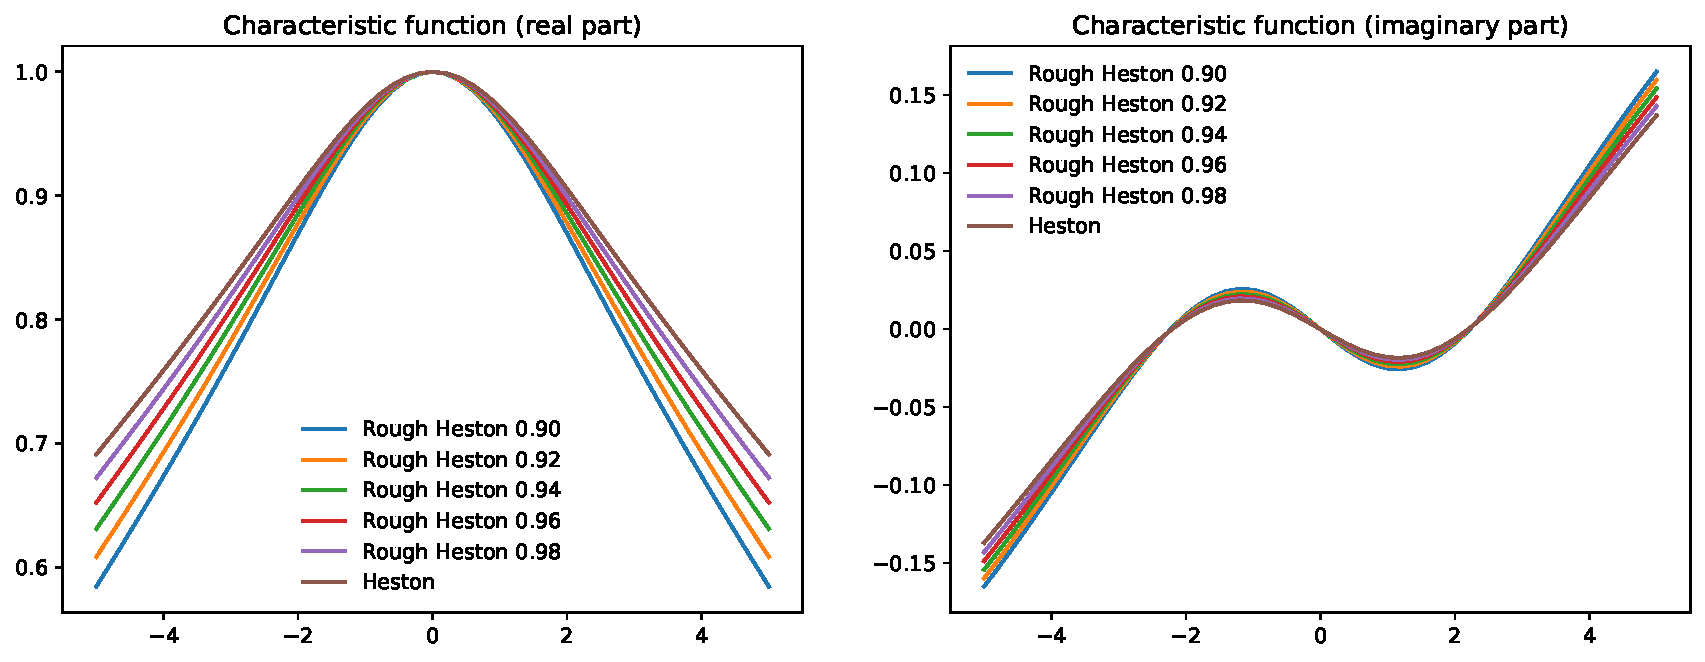
\includegraphics[width=1\textwidth]{figures/cf.pdf} \\
\caption{Real and imaginary part of the characteristic functions of the classical Heston model and Rough Heston model with different configurations of roughness parameter $\alpha$.}
\label{fig: characteristic function comparison}
\end{figure}

\subsubsection{Option pricing with transform methods}
\label{sec: option pricing with transform methods}

Recalling discussion from Section \ref{sec: characteristic function rough heston} we point out once again owning to its affine structure the Rough Heston model features semi-closed formula for the characteristic function identified by the fraction Riccati equation \eqref{eq: fractional riccati formulation}. Models with closed or semi-closed formula for characteristic function lend themselves to option pricing by transform methods which reduces computational time. In the following we elaborate on the pricing formulae described in \cite{CM99}.

We fix the timescale $T>0$ corresponding to option maturity. We write $f(u) = \mathbb E \left[ e^{iu \log S_T}\right]$ for the characteristic function of $\log S_T$. We work with the log-strike $k=\log K$ and consider the call option price $C(k) = \mathbb E \left[ (S_T - e^k)_+ \right]$. 

\paragraph{Fourier transform of the call price}

We want to consider the Fourier transform of the call option price $C(k)$. However, Fourier transform of the call option price does not exist since $C(k)\rightarrow \infty$ as $k\rightarrow -\infty$. Hence we need to consider the ``damped'' option price. We use the following convention for the Fourier transform.

\begin{definition}

The one-dimensional Fourier transform of a Lebesgue integrable function $f \in L^{1}\left(\mathbb{R}^{n}\right)$ and its inverse are given by

$$
\begin{aligned}
\hat{f}(\xi)&=\int_{-\infty}^{\infty} f(x) e^{-i x \xi} d x \\[10pt]
f(x)&=\frac{1}{2\pi}\int_{-\infty}^{\infty} \hat{f}(\xi) e^{i x \xi} d \xi.
\end{aligned}
$$

\end{definition}

\begin{lemma}

For the option price $C(k)$ we have for any $p>0$ the bounds

\begin{equation}
\label{eq: call price bounds}
\begin{aligned}
C(k) &\leqslant \frac{B_{0} \mathbb{E} \left[\exp ((p+1) \log S_T)\right]}{(p+1) \exp (p k)}\left(\frac{p}{p+1}\right)^{p} \\[10pt]
C(k) & \leqslant B_{0} \mathbb{E}\left[ S_T\right]
\end{aligned}
\end{equation}

\end{lemma}

\begin{proof}

It holds for all $s > 0$

$$
s - e^k \leq \frac{s^{p+1}}{(p+1) \exp (p k)}\left(\frac{p}{p+1}\right)^{p}
$$

since the left-hand side and right-hand side have the same value and first derivative at $s=(p+1) \exp (k) / p$ and second derivative of the right-hand side is everywhere positive. Making use of $(s - e^k)_+ \leq s-e^k$, replacing $s$ with $\log S_T$ and taking expectations yields the first inequality. The second bound is trivial.

\end{proof}

As we mentioned before, the option price does not decay as $k\rightarrow -\infty$. Hence Fourier transform of $C$ does not exist. We therefore introduce the damping constant $\theta > 0$ in order for the Fourier transform to exist:

$$
c_\theta(k) := \exp(\theta k) C(k).
$$

The damped call option price can be used to calculate the actual call option price with Fourier transform.

\begin{proposition}

For the call option price $C(k) = \mathbb E \left[(S_T-e_k)_+\right]$ we have

\begin{align}
C(k)&= \frac{\exp(-\theta k) }{\pi} \int_0^\infty \Re \left[ e^{-iuk} \hat c _\theta (u) \right] du \label{eq: fourier call price}\\[10pt]
\hat c _\theta (u) &= \frac{f(-u+i(\theta+1))}{\theta^{2}+2 \theta i u-u^{2}+\theta+i u}.
\end{align}


\end{proposition}

\begin{proof}

Bounds in \eqref{eq: call price bounds} imply that $c_\theta(k)$ decays exponentially for $k\rightarrow \pm \infty$. Since $c(k)$ is also bounded, it is in $L^1$ and has a Fourier transform.

With Fubini theorem we obtain the Fourier transform of the damped option price

\begin{equation}
\label{eq: fourier call calculation}
\begin{aligned}
\hat c_{\theta} (u) &= \int _{\infty} ^\infty e ^ {iuk} c _\theta(k) dk \\[5pt]
&= \int _{0} ^\infty \int _{-\infty} ^\infty (e^x-e^k)_+ e^{(\theta + ui)k}  dk dx \\[5pt]
&= \int _{-\infty} ^\infty e^{(\theta + iu)k} \left( \int_k^\infty(e^x-e^k) f(x)dx\right)dk\\[5pt]
&= \int _{-\infty} ^\infty e^x f(x) \int _{-\infty} ^x e^{(\theta + iu) k} dk dx - \int _{-\infty} ^\infty e^k f(x) \int _{-\infty} ^x e^{(\theta + iu) k} dk dx \\[5pt]
&= \int _{-\infty} ^\infty \frac{e^{(\theta + iu +1 )x}}{\theta + iu} f(x) dx - \int _{\infty} ^\infty \frac{e^{(\theta + iu +1 )x}}{\theta + iu + 1} f(x) dx \\[5pt]
&= \left(\frac{1}{\theta + iu} - \frac{1}{\theta + iu + 1} \right) \mathbb E \left[e^{(\theta + iu + 1)\log S_T} \right] \\[5pt]
&= \frac{f(-u +i (\theta + 1))}{\theta ^ 2 + 2\theta iu - u^2 + \theta+ iu}.
\end{aligned}
\end{equation}


The damped call option price is continuous and the transform is $L^1$ since

$$
|\hat c _\theta(u)| \leq \frac{\left|f\left(-\left(\theta+1\right) i\right)\right|} {\left(u^{2}+\theta^{2}\right)}.
$$

Hence the option price can be recovered by the inverse Fourier transform

$$
\begin{aligned}
C(k) &= \exp(-\theta k) c(k) \\[10pt]
&= \frac{\exp(-\theta k) }{2 \pi} \int_{-\infty}^\infty e^{-iuk} \hat c _\theta (u) du  \\[10pt]
&= \frac{\exp(-\theta k) }{\pi} \int_0^\infty \Re \left[ e^{-iuk} \hat c _\theta (u) \right] du.
\end{aligned}
$$

The last equation results from the complex conjugation.

\end{proof}

\begin{remark}
Note that positive values of $\theta$ facilitate integration as $k \rightarrow -\infty$, while negative values of $\theta$ ensure decay of the call price in the opposite direction $k \rightarrow + \infty$. Thus a calculation along the lines of \eqref{eq: fourier call calculation} implies that for the negative values of $\theta$ we recover put prices with the same formula.
\end{remark}

We also point out that while positive values of $\theta$ ensure that the call price decays for negative log-strikes and facilitate integration of \eqref{eq: fourier call price} as $k\rightarrow - \infty$, they impair integrability in the opposite direction $k \rightarrow +\infty$. In order for the call price to be integrable on the entire real line, it is sufficient to satisfy the upper bound

$$
\mathbb{E} \left[S_{T}^{\theta+1}\right]<\infty.
$$

Optimal choice of the damping parameter $\theta$ is all the more important for the calculation of the implied volatilities for extreme strikes. Consider example of a call option which pays $(S_T-K)_+$ at maturity. Price of a call option consists of the intrinsic value corresponding to its payoff $(S_T-K)_+$ at maturity and time value of the option corresponding to potential future earnings due to volatility in the spot price. Time value of the option is sensitive to volatility (typically grows as the volatility grows) while the intrinsic value is not.

Figure \ref{fig: intrinsic and time value of the option} demonstrates a typical pattern of intrinsic and time values of a call option. The difference of the actual option price and the intrinsic value is the time value of the option.

\begin{figure}[H]
\centering
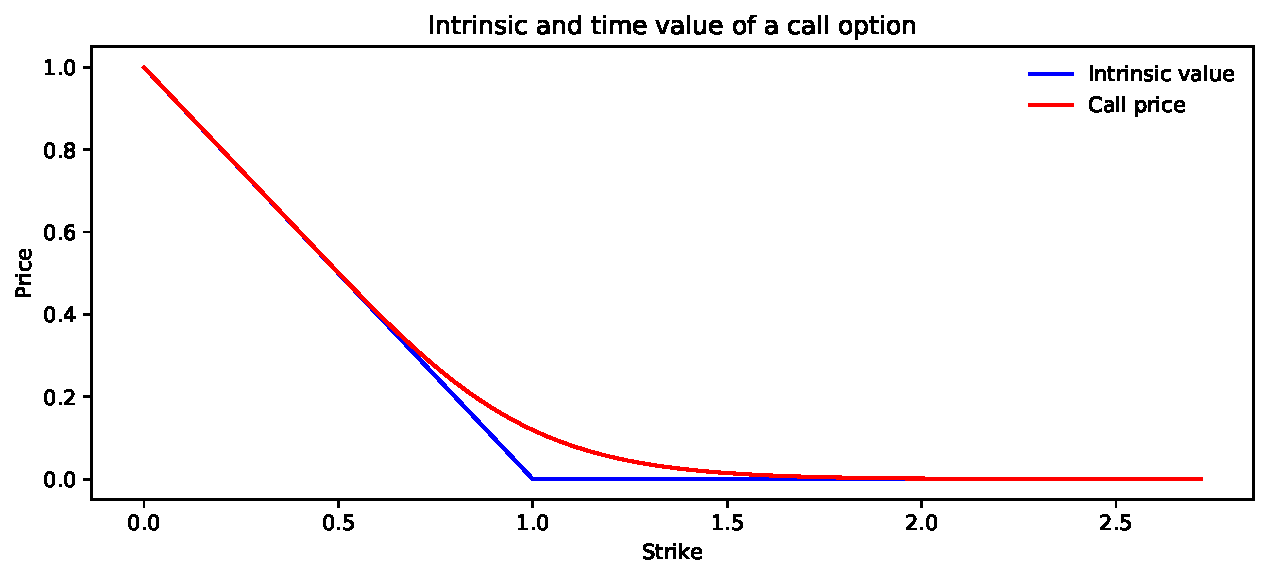
\includegraphics[width=0.8\textwidth]{figures/intrinsic.pdf} \\
\caption{Intrinsic and time value of a call option struck at $K=1$.}
\label{fig: intrinsic and time value of the option}
\end{figure}

For deep in-the-money options we have $C\approx S_T$ and for the deep out-of-the-money options we have $C\approx 0$. Thus for deep-in-the-money options sensitivity to volatility is negligible in relative terms (large changes in volatility barely affect the call price $C\approx S_T$) and it is more challenging to imply volatilities \eqref{eq: black scholes iv} using the deep-in-the-money options. On the other hand, for deep out-of-the-money options the intrinsic value of the option is zero and their price reflects the solely time value of the option, whence it is easier to imply volatility. Thus deep out-of-the-money puts should be used for the calculation of the implied volatilities for negative log-strikes instead.

Accordingly, appropriate choice of the damping constant $\theta$ is imperative to avoid negative option prices at extreme strikes and ensure that a root-finding procedure solving \eqref{eq: black scholes iv} produces reasonable implied volatility smile.

\paragraph{Option pricing with fast Fourier transform}

In order to efficiently compute the integral \eqref{eq: fourier call price}, we want to rewrite it in terms of the discrete Fourier transform. It would allow us to apply the fast Fourier transform algorithm (FFT). Fast Fourier transform is a divide-and-conquer type of algorithm that elegantly uses roots of unity to reduce the calculation time from an order of $O(N^2)$ to an order of $O(N\log N)$.

\begin{definition}
For a vector $x(j)$ with $j \in \{1, \dots, N\}$ the \emph{discrete Fourier transform (DFT)} is given by

\begin{equation}
\label{eq: dft}    
w(k)=\sum_{j=1}^{N} \mathrm{e}^{-\mathrm{i} \frac{2 \pi}{N}(j-1)(k-1)} x(j) \quad \text { for } k=1, \ldots, N.
\end{equation}

\end{definition}

We now aim to rewrite the integral \eqref{eq: fourier call price} corresponding to the option price in the shape of discrete Fourier transform \eqref{eq: dft}. Note that the integral can be discretized

$$
C_{T}(k) \approx \frac{\exp (-\theta k)}{\pi} \sum_{j=1}^{N} e^{-i v_{j} k} \psi_{T}\left(v_{j}\right) \eta
$$

with the step size $\eta$ and $v_{j}=\eta(j-1)$ for $j \in \{1, \dots, N\}$. We consider a range of log-strikes with spacing $\lambda > 0$

$$
k_{u}=-b+\lambda(u-1) \quad \text { for } u=1, \ldots, N
$$

\vspace{5pt}

for $b=\frac{1}{2} N \lambda$ and aim to calculate call prices 

$$
C_{T}\left(k_{u}\right) \approx \frac{\exp \left(-\theta k_{u}\right)}{\pi} \sum_{j=1}^{N} e^{-i v_{j}[-b+\lambda(u-1)]} \psi_{T}\left(v_{j}\right) \eta \quad \text { for } u=1, \ldots, N
$$

By construction, the set of log-strikes $k_u$ ranges from $-b$ to $b$. We can plug in $v_{j}=(j-1) \eta$ and set a constraint

\begin{equation}
\label{eq: fourier reciprocity relation}
\lambda \eta=\frac{2 \pi}{N}
\end{equation}

to obtain the call price in the form of discrete Fourier transform

$$
\begin{aligned}
C_{T}\left(k_{u}\right) &\approx \frac{\exp \left(-\theta k_{u}\right)}{\pi} \sum_{j=1}^{N} e^{-i \lambda \eta(j-1)(u-1)} e^{i b v_{j}} \psi_{T}\left(v_{j}\right) \eta \\[5pt]
&= \frac{\exp \left(-\theta k_{u}\right)}{\pi} \sum_{j=1}^{N} e^{-i \frac{2\pi}{N} (j-1)(u-1)} e^{i  b v_{j}} \psi_{T}\left(v_{j}\right) \eta.
\end{aligned}
$$

In the procedure above the number of the log-strikes computed and the grid spacing are coupled by the reciprocity relation \eqref{eq: fourier reciprocity relation}. Thus in order to increase the calculation precision one needs to incorporate more call prices. However, computational advantage created by fast Fourier transform is so significant that calculation of a larger number of call prices with fast Fourier transform algorithm is often considerably faster than calculating the sums \eqref{eq: dft} directly.

\subsection{Implied variance asymptotics}

In order to ensure that our implementation is correct, we first perform a sanity check by reconciling the classical Heston implied variance asymptotics from \cite{FGGS10} with the asymptotics obtained in \eqref{eq: left wing implied volatility asymptotics} and \eqref{eq: right wing implied volatility asymptotics}.

Figure \ref{fig: asymptotic rough heston reconciliation} shows the variance smiles of the Heston model and Rough Heston model with $\alpha=0.999$ generated by matching the implied volatility of options priced with transform methods as elaborated in Section \ref{sec: option pricing with transform methods}. As suggested before, we use out-of-the-money call options for positive log-strikes and out-of-the-money put options for negative log-strikes to imply volatilities. We use explicit formulae from \cite{H93} for the characteristic function of the Heston model. The characteristic function of the Rough Heston model was calculated by means of the fractional Adams method described in Section \ref{sec: numerical scheme of characteristic function}.

\begin{figure}[H]
\centering
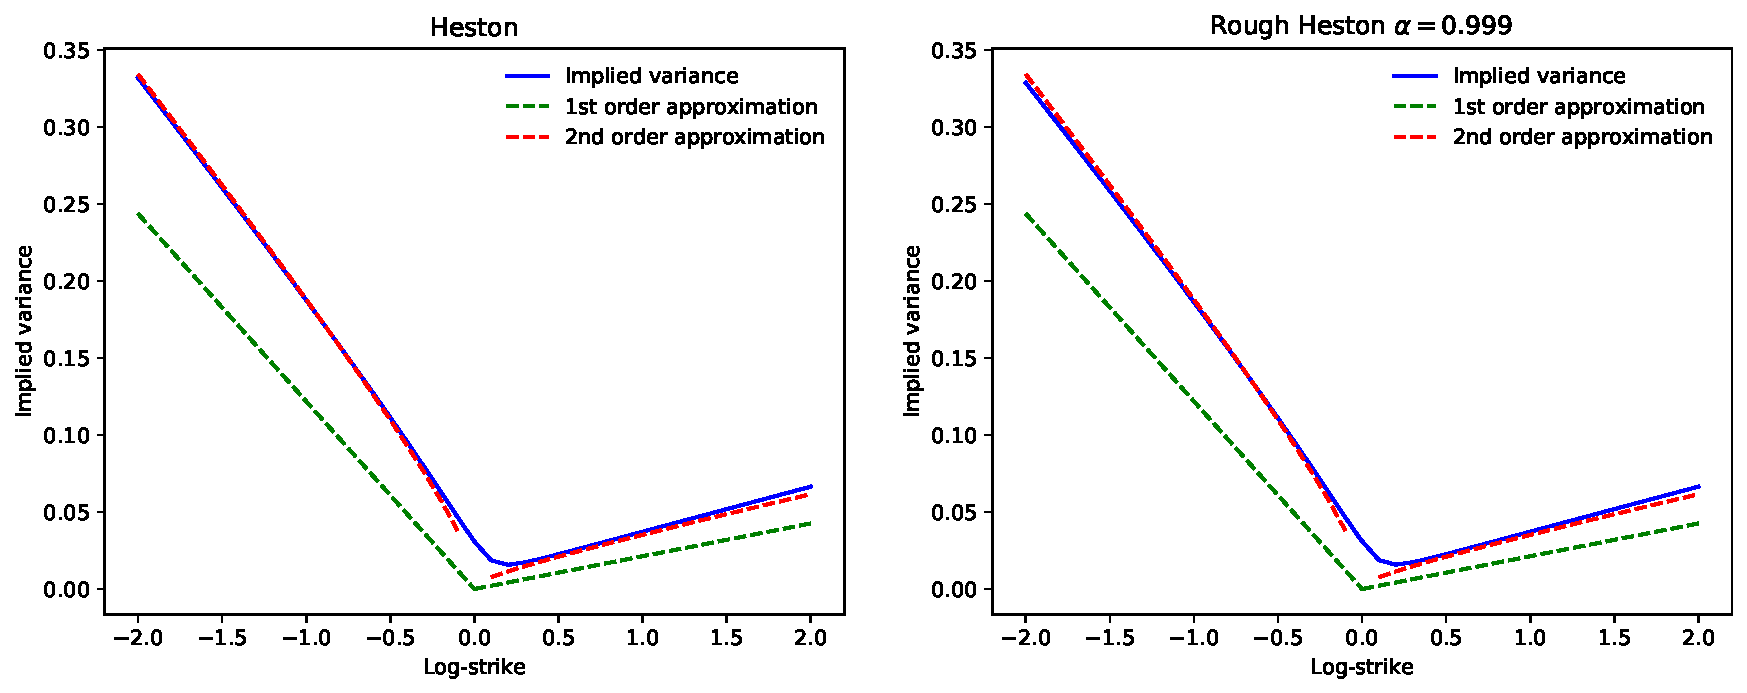
\includegraphics[width=1\textwidth]{figures/reconciliation.pdf} \\
\caption{Variance smile, first-order asymptotic and second-order asymptotics of the classical Heston model and Rough Heston model with $\alpha=0.999$.}
\label{fig: asymptotic rough heston reconciliation}
\end{figure}

The leading order approximation in the Figure \ref{fig: asymptotic rough heston reconciliation} is given by the Lee's moment formula \cite{L03} which establishes one-to-one correspondence between tail slope and finite moments of the log-spot. The first-order implied variance asymptotic for large strikes reads

$$
\sigma_{B S}(k, T)^{2} T \sim \Psi\left(s_{+}-1\right) \times k
$$

\vspace{10pt}

where $\Psi(x) = 2 - 4 (\sqrt{x^2-x} - x)$. The higher-order expansion of the left and right wing of the implied variance smile in the classical Heston model has been obtained in \cite{FGGS10} and is given by

$$
\sigma_{B S}(k, T)^{2} T=\left(\beta^\pm_{1} k^{1 / 2}+\beta^\pm_{2}+\beta^\pm_{3} \frac{\log k}{k^{1 / 2}}+O\left(\frac{1}{k^{1 / 2}}\right)\right)^{2}
\qquad \text{ as } \qquad k \rightarrow \pm \infty
$$

where $\beta^\pm_1, \beta^\pm_2$ and $\beta^\pm_3$ are corresponding constants of the classical Heston model. Equivalent higher-order expansion of the implied variance smile in the Rough Heston model is given by \eqref{eq: right wing implied volatility asymptotics}.

It is evident from Figure \ref{fig: asymptotic rough heston reconciliation} that the Rough Heston model with $\alpha=0.999$ practically recovers the results of the classical Heston model (correspoding to $\alpha = 1$) obtained in \cite{FGGS10}, and we conclude that our implementation satisfies the limiting case.

Having established robustness of our implementation, we roughen the model by setting $\alpha = 0.9$ all other things equal. Figure \ref{fig: asymptotic rough heston 0.9} demonstrates the Rough Heston implied variance smile and corresponding smile asymptotics. We conclude that the second-order approximation provides significant improvement over the first-order asymptotics and allows for more accurate modelling of the volatility smile at extreme strikes.

\newpage\clearpage

\begin{figure}[H]
\centering
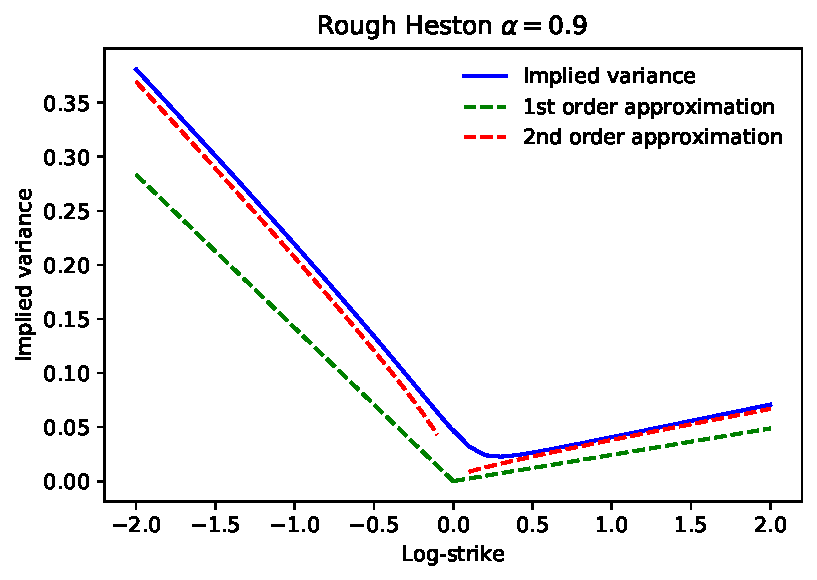
\includegraphics[width=0.7\textwidth]{figures/asymptotics.pdf} \\
\caption{Variance smile, first-order asymptotic and second-order asymptotic of the Rough Heston model with $\alpha=0.9.$}
\label{fig: asymptotic rough heston 0.9}
\end{figure}

\section{Conclusion}
\label{sec: conclusion}

In this thesis we have obtained a refined asymptotic expansion of the marginal density in the Rough Heston model. The analysis relies on the asymptotic expansion of the Volterra integral equation near explosion. Asymptotic approximation of the marginal density is subsequently obtained with the saddlepoint method. The results feature expansion of the Rough Heston marginal density at infinity and near the origin. As anticipated, asymptotics of the density factorize into leading order power law and a slowly varying function. Constants in the asymptotic expansion of the density depend solely on model parameters, the critical moment $s_\pm$ and the critical slope $\sigma_\pm$.

The marginal density asymptotics translate naturally to higher-order asymptotics of the implied variance smile. The obtained approximations demostrate a better fit for the implied volatility smile asymptotics than the first-order approximation with Lee's moment formula. Therefore, the results allow for more accurate modelling of volatility surface at extreme strikes.

Importantly, the results generalize equivalent asymptotic expansions for the classical Heston case. In particular, with the Hurst parameter $H = \frac 12$ the results are conformal with the analysis of the classical Heston model in \cite{FGGS10}.

The verification of the assumptions imposed on the asymptotic expansion of the solution of the fractional Riccati equation listed in Remark \ref{remark: assumptions} and assumptions concerning differentiability of the critical time in the Rough Heston model in Proposition \ref{prop: explosion in terms of the critical moments} is left for future investigation. They would entail further examination of the blow-up behavior of the Volterra integral equation \eqref{eq: original volterra equation}. 

\newpage

\printbibliography

\newpage

{\Large\textbf{Declaration of Authorship}}

I hereby confirm that I, Konstantins Starovoitovs, have authored this master thesis independently and without use of others than the indicated sources. Where I have consulted the published work of others, in any form (e.g. ideas, equations, figures, text, tables), this is always explicitly attributed.
\vspace{1cm}

July 2, 2020 \\ Berlin
\vspace{0.5cm}


Konstantins Starovoitovs

\vspace{70pt}

{\Large\textbf{Eidesstattliche Erklärung}}

Hiermit erkläre ich, Konstantins Starovoitovs, dass ich die vorliegende Arbeit allein und nur unter Verwendung der aufgeführten Quellen und Hilfsmittel angefertigt habe. Die Prüfungsordnung ist mir bekannt. Ich habe in meinem Studienfach bisher keine Masterarbeit eingereicht bzw. diese nicht endgültig nicht bestanden.

\vspace{1cm}

2. Juli 2020 \\ Berlin
\vspace{0.5cm}



Konstantins Starovoitovs


\end{document}
